%%%%%%%%%%%%%%%%%%%%%
% Documento maestro %
%%%%%%%%%%%%%%%%%%%%%
\documentclass{fime}

%%%%%%%%%%%%%%%%%%%%%%%%%%%%%%%%%%%%%%%%%%%
% Cargando paquetes y definiendo opciones %
%%%%%%%%%%%%%%%%%%%%%%%%%%%%%%%%%%%%%%%%%%%
% Aquí puedes cargar los paquetes que vas a usar. La clase
% fime ya incluye babel, inputenc, graphicx y los de la AMS.
% Cargar un paquete está a tu libertad (y responsabilidad).
\usepackage{algorithm} 
\usepackage{algpseudocode} 
\usepackage{listings}
\usepackage[flushleft]{threeparttable}

\usepackage{hyperref}
\usepackage{graphicx}
\usepackage{subfig}
\usepackage{pdflscape}
\usepackage[numbers,sort&compress]{natbib}
\usepackage{float}
\usepackage{footmisc}
\usepackage{adjustbox}
\usepackage{tikz}
\usepackage{listing}
\usepackage{pythonhighlight}
\usepackage{rotating}
\usepackage{array,booktabs,makecell}
\usetikzlibrary{arrows, babel, shapes}
\usepackage[font=small, skip=0pt]{caption}
\setlength{\footnotesep}{0.5cm}
\setlength\footnotemargin{3pt}
\hypersetup{breaklinks=true,colorlinks=true,    linkcolor=black,citecolor=black,urlcolor=black}
\usepackage[nodisplayskipstretch]{setspace}
\setstretch{1.5}
\tikzstyle{decision} = [diamond, draw, fill=yellow!20, text width=8em, text badly centered, node distance=3.5cm, inner sep=0pt]
\tikzstyle{block} = [rectangle, draw, fill=blue!20, text width=12em, text centered, rounded corners, minimum height=4em]
\tikzstyle{line} = [draw, -latex']
\tikzstyle{cloud} = [draw, ellipse,fill=red!20, node distance=1cm,minimum height=4em, text width=4em, text centered]

\renewcommand{\lstlistingname}{Código}
\renewcommand{\lstlistlistingname}{Lista de \lstlistingname s}

\makeatletter
\renewcommand*{\ALG@name}{Algoritmo}
\makeatother
\renewcommand{\tablename}{Cuadro}
\renewcommand{\arraystretch}{1.4}


% Caracteres usados en código 
\lstset{
    language=Python,
    literate={á}{{\'a}}1
        {ã}{{\~a}}1
        {é}{{\'e}}1
        {ó}{{\'o}}1
        {í}{{\'i}}1
        {ñ}{{\~n}}1
        {¡}{{!`}}1
        {¿}{{?`}}1
        {ú}{{\'u}}1
        {Í}{{\'I}}1
        {Ó}{{\'O}}1
}
% Estilo de código
\definecolor{codegreen}{rgb}{0,0.6,0}
\definecolor{codegray}{rgb}{0.5,0.5,0.5}
\definecolor{codepurple}{rgb}{0.58,0,0.82}
\definecolor{backcolour}{rgb}{0.95,0.95,0.92}
\lstdefinestyle{pys}{
    backgroundcolor=\color{white},   
    commentstyle=\color{codegreen},
    keywordstyle=\bfseries\color{blue},
    numberstyle=\tiny\color{codegray},
    stringstyle=\color{codepurple},
    basicstyle=\tiny,
    breakatwhitespace=false,         
    breaklines=true,                 
    captionpos=b,                    
    keepspaces=true,                 
    numbers=left,                    
    numbersep=25pt,                  
    showspaces=false,                
    showstringspaces=false,
    showtabs=true,                  
    tabsize=2
}
\lstset{style=pys}


%%%%%%%%%%%%%%%%%%%%%
% Definiendo campos %
%%%%%%%%%%%%%%%%%%%%%
\def\titulo{Modelado y visualización de relaciones entre contaminantes del aire y salud pública}
\def\autor{Selene Berenice Prado Prado}
\def\matricula{1810042}
\def\grado{Ingeniería en Tecnología de Software}
% En caso de que el grado tenga orientación o especialidad llenar el siguiente
% campo dejando un ESPACIO INICIAL, en caso contrario, dejar vacío
\def\orientacion{}
\def\fecha{Julio 2022} % Coloca el mes con mayúscula inicial

\def\asesor{Dra. Satu Elisa Schaeffer}
\def\revisorA{Dra. Sara Elena Garza Villarreal}
\def\revisorB{Dr. José Arturo Berrones Santos}
% En el caso de que tu tesis sea de doctorado activa la variable cambiándola a \doctoradotrue
% y define tus otros dos revisores
\newif\ifdoctorado\doctoradofalse
\def\revisorC{Nombre del revisor C}
\def\revisorD{Nombre del revisor D}
% El visto bueno siempre va
\def\vobo{Dr. Fernando Banda Muñoz}

%%%%%%%%%%%%%%%%%%%%%%%
% Inicia el documento %
%%%%%%%%%%%%%%%%%%%%%%%
\begin{document}

\frontmatter
\pagestyle{main}

%%% Incluye PortillasM si tu tesis es de Maestría
%%% y PortillasD si es de doctorado.
% Portadas (Maestría)

\def\uanl{Universidad Autónoma de Nuevo León}
\def\fime{Facultad de Ingeniería Mecánica y Eléctrica}
\def\depg{Subdirección Académica}
\def\snnl{San Nicolás de los Garza, Nuevo León}

%%%%%%%%%%%%%%%%%%%%%%%%
% Primer portada: UANL %
%%%%%%%%%%%%%%%%%%%%%%%%
\thispagestyle{empty}

\begin{scshape}
\begin{center}
	{\Large \uanl} \\[5mm]
	{\large \fime} \\[5mm]
	{\large \depg}
	\vskip 15mm
	
\includegraphics[height=55mm]{uanl}
	\vskip 12mm
	\begin{tabular}{p{11cm}}
		\centering
		{\large \titulo}
	\end{tabular}
	\vskip 7mm
	{por}\\[7mm]
	{\large \autor}\\[7mm]
	{como requisito parcial para obtener el grado de}\\[3mm]
	\MakeUppercase{\grado}\\
	\orientacion
	\vfill
	\fecha
\end{center}
\end{scshape}

%%%%%%%%%%%%%%%%%%%%%%%%%
% Segunda portada: FIME %
%%%%%%%%%%%%%%%%%%%%%%%%%
\newpage
\thispagestyle{empty}

\begin{scshape}
\begin{center}
	{\Large \uanl} \\[5mm]
	{\large \fime} \\[5mm]
	{\large \depg}
	\vskip 16mm
	
\includegraphics[height=50mm]{fime}
	\vskip 16mm
	\begin{tabular}{p{11cm}}
		\centering
		{\large \titulo}
	\end{tabular}
	\vskip 7mm
	{por}\\[7mm]
	{\large \autor}\\[7mm]
	{como requisito parcial para obtener el grado de}\\[3mm]
	\MakeUppercase{\grado}\\
	\orientacion
	\vfill
	\fecha
\end{center}
\end{scshape}

%%%%%%%%%%%%%%%%%%%%%%%%%%%%%
% Carta del comité de tesis %
%%%%%%%%%%%%%%%%%%%%%%%%%%%%%
\newpage
\thispagestyle{empty}
\enlargethispage{5mm}

\begin{center}
{\bf \large \uanl} \\
{\bf \fime} \\
{\bf \depg}
\end{center}
\vskip 4mm

Los miembros del Comité de Tesis recomendamos que la Tesis <<\titulo>>, realizada por el alumno \autor, con número de matrícula \matricula, sea aceptada para su defensa como requisito parcial para obtener el grado de \grado\orientacion.
\ifdoctorado{\vskip 10mm}\else{\vskip 8mm}\fi

\begin{center}
El Comité de Tesis\\
\ifdoctorado{\vskip 15mm}\else{\vskip 25mm}\fi

\ifdoctorado{%%%
\begin{tabular}{p{37mm}p{21mm}p{12mm}p{21mm}p{37mm}}
	\cline{2-4}
	& \multicolumn{3}{c}{\asesor} & \\
	& \multicolumn{3}{c}{Asesor}  & \\[15mm]
	\cline{1-2} \cline{4-5}
	\multicolumn{2}{c}{\revisorA} & & \multicolumn{2}{c}{\revisorB} \\
	\multicolumn{2}{c}{Revisor}   & & \multicolumn{2}{c}{Revisor}   \\[17mm]
	\cline{1-2} \cline{4-5}
	\multicolumn{2}{c}{\revisorC} & & \multicolumn{2}{c}{\revisorD} \\
	\multicolumn{2}{c}{Revisor}   & & \multicolumn{2}{c}{Revisor}   \\[2mm]
	& \multicolumn{3}{c}{Vo. Bo.} & \\[14mm]
	\cline{2-4}
	& \multicolumn{3}{c}{\vobo}   & \\
	& \multicolumn{3}{c}{\depg}   & \\ &&&&
\end{tabular}
}\else{%%%
\begin{tabular}{p{37mm}p{21mm}p{12mm}p{21mm}p{37mm}}
	\cline{2-4}
	& \multicolumn{3}{c}{\asesor} & \\
	& \multicolumn{3}{c}{Asesora}  & \\[19mm]
	\cline{1-2} \cline{4-5}
	\multicolumn{2}{c}{\revisorA} & & \multicolumn{2}{c}{\revisorB} \\
	\multicolumn{2}{c}{Revisora}   & & \multicolumn{2}{c}{Revisora}   \\[2mm]
	& \multicolumn{3}{c}{Vo. Bo.} & \\[17mm]
	\cline{2-4}
	& \multicolumn{3}{c}{\vobo}   & \\
	& \multicolumn{3}{c}{\depg}   & \\ &&&&
\end{tabular}
}\fi%%%

\vfill

\snnl, \MakeLowercase{\fecha}

\end{center}

%%%% Dedicatoria

\thispagestyle{empty}
\vspace*{17mm}

\begin{flushright}
\begin{itshape}

Aquí puedes poner tu dedicatoria\\
si es que tienes una.\bigskip\bigskip

Si no tienes una, puedes borrar\\
la línea \verb+% Dedicatoria

\thispagestyle{empty}
\vspace*{17mm}

\begin{flushright}
\begin{itshape}

Aquí puedes poner tu dedicatoria\\
si es que tienes una.\bigskip\bigskip

Si no tienes una, puedes borrar\\
la línea \verb+% Dedicatoria

\thispagestyle{empty}
\vspace*{17mm}

\begin{flushright}
\begin{itshape}

Aquí puedes poner tu dedicatoria\\
si es que tienes una.\bigskip\bigskip

Si no tienes una, puedes borrar\\
la línea \verb+\include{Dedicatoria}+ en el\\
archivo \texttt{MiTesis.tex} pues no es obligatoria.

\end{itshape}
\end{flushright}

+ en el\\
archivo \texttt{MiTesis.tex} pues no es obligatoria.

\end{itshape}
\end{flushright}

+ en el\\
archivo \texttt{MiTesis.tex} pues no es obligatoria.

\end{itshape}
\end{flushright}



\tableofcontents
\listoffigures
\listoftables

%Agradecimientos

\chapter{Agradecimientos}
\markboth{Agradecimientos}{}

Quiero agradecer a la Dra. Elisa, por el apoyo, el conocimiento y el tiempo que invirtió durante el desarrollo de mi tesis para poder hacer una gran investigación. Al Dr. Manuel Jiménez, por el material brindado además de los aportes que hizo para complementar la tesis y al Fondo Sectorial de Investigación Ambiental SEMARNAT-CONACYT con No. de proyecto 263080.

A mis padres, José Angel y Bertha Alicia, quienes siempre me motivaron a seguir adelante y son el motor de mi vida. A mis hermanas y sobrinos por su gran apoyo en todo momento, a mis abuelos Sara y José Reyes que siempre me motivaron a crecer como persona y alcanzar la meta de superarme.

Mención especial a mi abuelo Reyes (QEPD), quien en todo momento, incluso meses antes de fallecer, siempre me apoyó y esperó que diera todo de mí para ser alguien mejor de lo que él fue.

%... debo mejorar esto, pero ya sé a quienes debo/quiero agradecer..
%Resumen

\chapter{Resumen}
\markboth{Resumen}{}

{\setlength{\leftskip}{10mm}
\setlength{\parindent}{-10mm}

\autor.

Candidato para obtener el grado de \grado\orientacion.

\uanl.

\fime.

Título del estudio: \textsc{\titulo}.

\noindent Número de páginas: \pageref*{lastpage}.}

%%% Comienza a llenar aquí
\paragraph{Objetivos y método de estudio:}
El objetivo de la investigación es generar modelos que permitan visualizar relaciones entre contaminantes atmosféricos y salud pública. Los modelos generados se utilizan en conjunto con datos obtenidos de la Secretaría de Salud del Gobierno de México y registros de los niveles de los contaminantes presentes en el área metropolitana de Monterrey. 

El tener un modelo que permita visualizar relaciones entre contaminantes atmosféricos y salud pública que sea utilizado con datos confiables y verídicos pueden ayudar a entender el impacto que tiene el aumento del nivel de contaminantes atmosféricos.
\paragraph{Contribuciones y conclusiones:}
En la investigación se exploran diversas maneras de visualizar la información, además de generar modelos que permiten analizar las relaciones existentes entre los niveles de determinados contaminantes y CIE. Las visualizaciones generadas son series de tiempo y gráficos de radar, y modelos de regresión lineal y de regresión lineal múltiple. 

\bigskip\noindent\begin{tabular}{lc}
\vspace*{-2mm}\hspace*{-2mm}Firma de la asesora: & \\
\cline{2-2} & \hspace*{1em}\asesor\hspace*{1em}
\end{tabular}

\bigskip\noindent\begin{tabular}{lc}
\vspace*{-2mm}\hspace*{-2mm}Firma de la coasesora: & \\
\cline{2-2} & \hspace*{1em}\revisorA\hspace*{1em}
\end{tabular}



\mainmatter
\pagestyle{fime}

%%% Haz un documento para cada capítulo
%\linenumbers
\chapter{Introducción}

El \emph{aprendizaje máquina}\footnote{Traducido como \emph{machine learning} en inglés, tiene como objetivo desarrollar técnicas que les permitan a las computadoras aprender.} es un área dentro de la \emph{ciencia de datos}\footnote{Traducido como \emph{data science} en inglés, involucra métodos para extraer conocimiento de datos, eso con la finalidad de que haya un mejor entendimiento de los datos.} que puede ayudar a crear dichos modelos para tener una más eficiente visualización cuando se trabaja con una gran cantidad de datos, que es lo que se requiere para el presente trabajo. El área de la ciencia de datos es muy útil ya que permite trabajar con grandes cantidades de datos aminorando la cantidad de tiempo empleado en la creación de gráficos que permitan visualizar los datos. El crear modelos para la visualización de datos ayuda a observar con mayor claridad los datos para encontrar relaciones entre ellos.


La tarea en el presente proyecto es utilizar modelos para visualizar las relaciones entre los contaminantes del aire y salud pública. Para la realización de los experimentos se tienen datos de ingresos hospitalarios provenientes de la base de datos de la Secretaría de Salud del Gobierno de México \cite{f1}. También se tienen registros de los niveles de algunos contaminantes del aire presentes en el área metropolitana de Monterrey, capturados por las estaciones de monitoreo pertenecientes al Sistema Integral de Monitoreo Ambiental (SIMA) \cite{f2} mostradas en la figura \ref{estaciones} y en el cuadro \ref{tab:Coordenadas estaciones}.

\begin{figure}[h!]
\setcounter{figure}{0} % por culpa de sciposter
\captionsetup{type=figure} % por culpa de sciposter
\begin{center}
   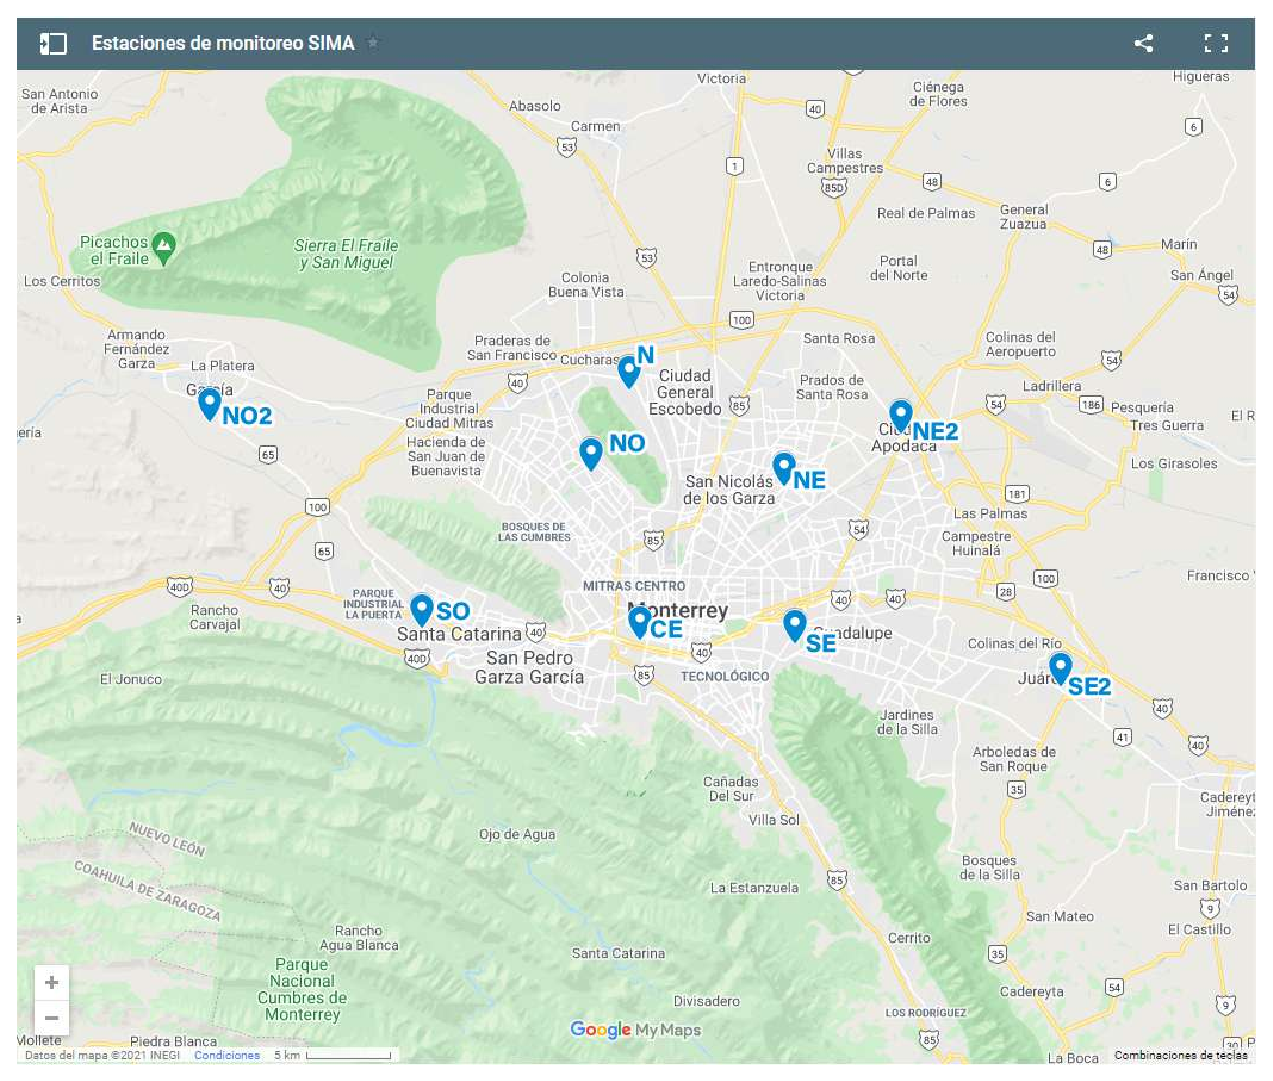
\includegraphics[trim=50 50 50 50,clip,width=1\textwidth]{mapa_estaciones.eps}
   \end{center}
    \caption{Localización de las estaciones de monitoreo de la calidad del aire.}
    \label{estaciones}
\end{figure}

%Las herramientas utilizadas en la presente investigación se muestran en el cuadro \ref{tab:Coordenadas estaciones}.
\begin{table}[H]
	{\centering
		\caption{Coordenadas de las estaciones de monitoreo de la calidad del aire.}
		\begin{tabular}{|c|c|c|}
			\hline 
			Estación & Latitud & Longitud\\
			\hline
			SE & 25.668 & -100.249\\
			\hline
			NE & 25.750 & -100.255\\
			\hline
			CE & 25.670 & -100.338\\
			\hline
			NO & 25.757 & -100.366\\
			\hline
			SO & 25.676 & -100.464\\
			\hline
			NO2 & 25.783 & -100.586\\
			\hline
			NE2 & 25.777 & -100.188\\
			\hline
			N & 25.800 & -100.344\\
			\hline
			SE2 & 25.646 & -100.096\\
			\hline
		\end{tabular}
		
	\label{tab:Coordenadas estaciones}
	}
\end{table}












\clearpage
\section{Motivación}
Existen investigaciones que ya han estudiado las relaciones entre contaminantes del aire y salud pública, sin embargo, con el presente trabajo se busca aportar a la creación de nuevas herramientas que permitan observar y estudiar dichas relaciones con el fin de ayudar a tomar medidas adecuadas que permitan aminorar los efectos negativos de los contaminantes del aire en la salud.

\section{Hipótesis}
Los modelos de regresión permiten obtener gráficos donde se pueden observar las relaciones entre el número de ingresos hospitalarios y los niveles de contaminantes del aire.

\section{Objetivos}
En esta sección se establece el objetivo general y los objetivos específicos sobre los que se orienta el presente trabajo.

\subsection{Objetivo general}
Generar, implementar y evaluar modelos que muestran las relaciones existentes entre contaminantes del aire y salud pública tiene la finalidad de apoyar a la implementación de estrategias que aminoran los efectos negativos de los contaminantes del aire en la salud de las personas. Con los modelos generados se puede tener una herramienta que permite identificar gráficamente las relaciones con solo proporcionarle el conjunto de datos.

\subsection{Objetivos específicos}
\begin{itemize}
\item Generar, implementar y evaluar modelos de regresión que permiten cuantificar las relaciones entre contaminantes del aire y salud pública a partir de un conjunto de datos.
\end{itemize}
\begin{itemize}
\item Diseñar e implementar visualizaciones interactivas que permiten explorar los modelos implementados y su validez estadística.
\end{itemize}
\begin{itemize}
\item Evaluar la eficacia de los modelos generados para tener noción de la fiabilidad del análisis realizado a partir de los resultados que tales modelos producen.
\end{itemize}
%\begin{itemize}
%\item Generar un modelo de regresión que permite estudiar las relaciones entre los niveles de contaminantes del aire y salud pública.
%\end{itemize}

%\section{Estructura}
%El contenido de la investigación se divide en...
\chapter{Antecedentes}

%En algunos trabajos se han utilizado modelos de series de tiempo y ...
Existen factores ambientales que afectan la salud de una comunidad como: el abastecimiento de agua potable y el saneamiento, la vivienda y el hábitat, la alimentación, la contaminación ambiental, el empleo de productos químicos y los riesgos ocupacionales \citep{r2}. 

Contaminación del aire es un término usado para describir la presencia de uno o más contaminantes en la atmósfera, cuyas cantidades y características pueden resultar perjudiciales o interferir con la salud, el bienestar u otros procesos ambientales naturales \citep{r3}.

En este capítulo se presentan los fundamentos y definiciones de los conceptos más relevantes para el tema de estudio abordado.
%\section{Antecedentes históricos}

\section{Monitoreo de calidad del aire}
Existen diversos estudios que muestran la existencia de potenciales efectos a la salud cuando en el aire están presentes contaminantes en forma de partículas, gases o agentes biológicos.
%En los últimos años ha habido un desarrollo considerable de la tecnología para el control de la calidad del aire, esto como resultado de una mayor conciencia, tanto de parte de los gobiernos como de los ciudadanos, sobre la importancia de mantener el aire lo más apto posible para la vida humana.

\citet{r4} mencionan que desde inicios de 1950 se observa una preocupación por los contaminantes del aire  en los países de América Latina y el Caribe. Las universidades y dependencias de los ministerios de salud fueron los organismos que realizaron las primeras mediciones de contaminación en el aire.

En 1965, el Consejo Directivo de la Organización Panamericana de la Salud (OPS) recomendó el establecer programas de investigación de la contaminación del agua y del aire, con el objetivo de colaborar en el desarrollo de políticas adecuadas de control \citep{r5}.

Mediante el Centro Panamericano de Ingeniería Sanitaria y Ciencias del Ambiente (CEPIS), la OPS acordó establecer una red de estaciones de muestreo de la contaminación del aire.
En junio de 1967 la Red Panamericana de Muestreo Normalizado de la Contaminación del Aire (REDPANAIRE) inició sus operaciones recolectando muestras diarias de partículas totales en suspensión (PTS) y de SO$_2$. La REDPANAIRE comenzó con ocho estaciones y a fines de 1973 tenía un total de 88 estaciones distribuidas en 26 ciudades de 14 países \citep{r5}.

Para diciembre de 1973 se habían recolectado más de 350,000 datos sobre la calidad del aire, en los que se observa que algunas ciudades mostraban una tendencia al incremento de los niveles de contaminación \citep{r5}.

En 1980 la REDPANAIRE desapareció y pasó a formar parte del Programa Global de Monitoreo de la Calidad del Aire, iniciado en 1976 por la OMS y el Programa de las Naciones Unidas para el Medio Ambiente (PNUMA), como parte de un sistema global de monitoreo ambiental llamado GEMS por sus siglas en inglés \emph{Global Environmental Monitoring System}.

En la década de 1990, la OMS instituyó, con carácter global, el Sistema de Información para el Control de la Calidad del Aire llamado AMIS por sus siglas en inglés \emph{Air Management Information System}. Entre las actividades más destacadas de AMIS se incluye el coordinar las bases de datos sobre temas relacionados con la calidad del aire.

En Nuevo León, México, las operaciones de la Red Automática de Monitoreo Atmosférico iniciaron en 1993. Dicha red en sus inicios contaba con cinco estaciones fijas de monitoreo continuo de monóxido de carbono (CO), dióxido de azufre (SO$_2$), óxidos de nitrógeno (NO$_x$), ozono (O$_3$) y partículas de tamaño menor a 10 micrómetros (PM10) \citep{r4}. Como se muestra en la figura \ref{estaciones} y en el cuadro \ref{tab:Coordenadas estaciones}, actualmente se cuenta con nueve estaciones fijas.

\section{Series de tiempo}
\citet{r4} mencionan que las relaciones entre niveles de concentraciones de contaminantes del aire y los efectos sobre la salud generalmente son obtenidas de estudios epidemiológicos de series de tiempo. Uno de los diseños epidemiológicos más utilizados son los estudios de series temporales. Con esos diseños se analizan las variaciones en el tiempo de la exposición al contaminante y el indicador de salud estudiado en una población \citep{r1}.

Las series de tiempo se pueden definir como un conjunto de observaciones ${{ot}}$ tomadas en un tiempo $t$ determinado. Los estudios de series de tiempo relacionan estadísticamente los cambios temporales en la repercusión de cambios en la concentración de un contaminante en la población \citep{r8}.

Para mostrar datos en una serie de tiempo, especialmente en el área médica, estos suelen agruparse en \emph{semanas epidemiológicas}\footnote{Una semana epidemiológica es un estándar de medición temporal que se utiliza para comparar datos en ventanas de tiempo definidas. La primera semana epidemiológica del año termina el primer sábado de enero de cada año \citep{r7}.}. El agrupamiento en semanas epidemiológicas a diferencia del agrupamiento traducido como \emph{clustering} en inglés que consiste en crear grupos de objetos con similitudes entre ellos a partir de datos no etiquetados, consiste en agrupar los objetos en semanas del año dependiendo de la fecha en que se registró el objeto.

\section{Clasificación de enfermedades}
Existe un instrumento estadístico y sanitario para identificar enfermedades llamado Clasificación Internacional de Enfermedades (CIE), cuya finalidad es entender las causas de morbilidad y mortalidad de la población y así mejorar la calidad de vida de la misma. Es en base a un criterio epidemiológico y sanitario establecido por Farr a finales del siglo XIX que esta clasificación agrupa enfermedades en epidémicas, generales, locales ordenadas por origen geográfico, trastornos del desarrollo y lesiones \citep{r9}. Para lograr distinguirlas se emplea un código alfanumérico que consiste de una letra en la primera posición, seguida de dos dígitos, un punto decimal y un último dígito. El rango de valores va de A00.0 a Z99.9.

\section{Regresión lineal}
La tendencia $w_0$ de una serie de tiempo puede ser obtenida a partir de una regresión lineal de la misma \citep{r10}. Una regresión lineal es una metodología inferencial supervisada que busca predecir valores $y$ dado un vector de variables de entrada $t$ por medio del ajuste de coeficientes $w$ de la función lineal 
\begin{equation}
    \hat{y}(t,w) = w_0 + w_1x_1 + ... + w_tx_t.
    \label{eq1}
\end{equation}

\section{Regresión lineal múltiple}
Un modelo de regresión múltiple es un modelo complemento de la regresión lineal simple, el cual tiene dos o más variables independientes $k$ que pueden influir en una variable dependiente $y$. \citet{r11} expresan la regresión múltiple mediante la siguiente ecuación:
\begin{equation}
    y = \beta_0 + \beta_1x_1 + ... + \beta_kx_k + \varepsilon.
    \label{eq2}
\end{equation}

%\section{Modelos ARIMA}
%Los modelos autorregresivos integrados de media móvil o ARIMA, por su abreviatura en inglés abarcan un catalogo de aproximaciones para el estudio de series de tiempo. 

%Los modelos ARIMA utilizan variaciones y regresiones de datos estadísticos con el fin de encontrar patrones para una predicción hacia el futuro. 


\chapter{Estado del arte}

En el presente capítulo se estudia literatura reciente relacionada con el presente trabajo, esto con el objetivo de revisar distintos métodos para resolver el problema planteado en el presente trabajo y, además, también revisar implementaciones similares para resolver problemas distintos. Lo anterior tiene la finalidad de comparar los trabajos revisados e identificar áreas de oportunidad en ellos.

En la primera sección, \emph{trabajos relacionados}, se recopilan obras con características relacionadas al presente trabajo, ya sean relacionados con el problema que se pretende resolver o con los métodos empleados para buscar su resolución.

En la segunda sección, \emph{análisis comparativo}, se comparan las distintas características de los trabajos revisados, de esa forma se pueden determinar las principales ventajas y desventajas de cada trabajo. 

Finalmente, en la tercera sección, \emph{áreas de oportunidad}, se realiza una conclusión acerca de los resultados obtenidos del análisis comparativo.

\section{Trabajos relacionados}
Se recopila literatura relacionada desde el año 2017 hasta el año 2021. En esta sección los trabajos se mencionan en orden cronológico tomando en cuenta su año de publicación.

\citet{r12} estudian la relación entre los niveles de contaminantes ambientales y la presencia de casos de enfermedades respiratorias en las consultas pediátricas. La variable dependiente analizada es la demanda en las consultas pediátricas por bronquiolitis, episodios de broncoespasmo y procesos respiratorios de vías altas. Como variables independientes se tienen los valores de contaminación ambiental. Se calculan coeficientes de correlación y regresión lineal múltiple.

\citet{r13} abordan la necesidad de monitoreo, control y predicción de la pendiente de los niveles de contaminantes del aire. Para abordar el problema de investigación utilizan modelos ARIMA. 

\citet{r14} estudian la asociación entre la exposición a largo plazo a la contaminación del aire y la metilación del ADN. Para ello realizan un estudio utilizando modelos de regresión lineal robustos para analizar la asociación entre la exposición al NO$_2$ y a las partículas PM10 y PM2.5.

\citet{r15} en su estudio abordan los niveles de contaminación del aire y su asociación con la presencia de presión sanguínea elevada en niños y adolescentes. La exposición a partículas PM10 y PM2.5 son estimadas con un modelo espacio-temporal. Son utilizados modelos lineales de efectos mixtos y modelos de regresión logística para investigar la asociación entre la exposición a partículas PM y presión sanguínea e hipertensión. 

\citet{r16} estudian la relación entre los niveles de contaminación del aire y la obesidad y problemas cardiometabólicos. Para dicho estudio emplean modelos de regresión lineal.

\citet{r17} examinan las asociaciones entre la exposición temprana a la contaminación del aire y la incidencia de asma y rinitis alérgica desde el nacimiento hasta la adolescencia. Para su estudio utilizan modelos de regresión.

\citet{r18} estudian la asociación entre la exposición temprana a los contaminantes del aire y los egresos hospitalarios por asma. Para su estudio aplican modelos de regresión logística para el análisis de datos. 

\citet{r19} abordan el estudio de la relación entre los niveles de contaminación del aire y el número de admisiones hospitalarias. Para ello se construye un modelo basado en la distribución de Poisson.

\citet{r20} estudian la relación entre la mortalidad del coronavirus (COVID-19) y la contaminación del aire. Para dicho estudio emplean un modelo de regresión lineal para establecer la relación entre los parámetros de la contaminación del aire (concentraciones de PM10 o PM2.5) y la variable de respuesta (porcentaje de mortalidad por unidad de casos reportados).

\clearpage
\section{Comparación de trabajos}
La mayoría de los trabajos encontrados emplean modelos de regresión lineal o modelos de predicción. Además, en todos los trabajos encontrados el problema tratado presenta una alta relación con el problema abordado en el presente trabajo de tesis. El análisis comparativo de los trabajos relacionados se hace en base de los siguientes puntos:

\begin{description}
\item[Modelos de regresión lineal:]{Son aquellos que ayudan a estudiar la relación entre una variable dependiente y una o más variables independientes.}
\end{description}

\begin{description}
\item[Modelos de predicción:]{Son aquellos que ayudan a hacer predicciones de una variable.}
\end{description}

\begin{description}
\item[Evaluación de modelos:]{Se refiere a la utilización de técnicas para evaluar la eficacia de los modelos generados.}
\end{description}

\begin{description}
\item[Estudio de contaminantes del aire:]{Se refiere a que el tema de estudio incluya uno o más contaminantes del aire.}
\end{description}

\begin{description}
\item[Estudio de problemas de salud:]{Se refiere a que el tema de estudio incluya uno o más problemas de salud.}
\end{description}

En el cuadro \ref{tab:Comparación de trabajos frente al desarrollado} se desglosan las características presentes  que se pueden encontrar en las investigaciones citadas y su relación con la investigación con la que se está trabajando actualmente.

\begin{table}[hbt!]
\centering
\caption[Comparación de trabajos]{Comparación de trabajos frente al desarrollado, donde $\checkmark$ indica que cumple con esta característica y  $\times$ no cumple con esta característica.}
\vspace{0.5cm}
\begin{adjustbox}{width=0.5\textwidth}
\begin{tabular}{|l|c|c|c|c|c|}
\hline
Trabajo & \rotatebox[origin=c]{90}{ Modelos de regresión lineal } & \rotatebox[origin=c]{90}{ Modelos de predicción } & \rotatebox[origin=c]{90}{ Evaluación de modelos } & \rotatebox[origin=c]{90}{ Estudio de contaminantes del aire } & \rotatebox[origin=c]{90}{ Estudio de problemas de salud }\\
	\hline
    \citet{r12} & \checkmark & $\times$ & $\times$ & \checkmark & \checkmark\\
    \hline
    \citet{r13} &  $\times$ & \checkmark & \checkmark & \checkmark & $\times$\\
    \hline
    \citet{r14} & \checkmark & \checkmark & $\times$ & \checkmark & \checkmark\\
    \hline
    \citet{r15} & \checkmark & \checkmark & $\times$ & \checkmark & \checkmark\\
	\hline    
    \citet{r16}& \checkmark & $\times$ & $\times$ & \checkmark & \checkmark\\
	\hline    
    \citet{r17} & $\times$ & \checkmark & \checkmark & \checkmark & \checkmark\\
	\hline    
    \citet{r18} & $\times$  & $\times$ & $\times$ & \checkmark & \checkmark\\
	\hline    
    \citet{r19} & \checkmark & \checkmark & $\times$ & \checkmark & \checkmark\\
	\hline    
    \citet{r20} &  \checkmark & \checkmark & $\times$ & \checkmark & \checkmark\\
	\hline    
    El presente trabajo & \checkmark & \checkmark & \checkmark & \checkmark & \checkmark\\
    \hline
\end{tabular}
\end{adjustbox}
\label{tab:Comparación de trabajos frente al desarrollado}
\end{table}

\clearpage
\subsection{Áreas de oportunidad}
Como se puede observar en el cuadro \ref{tab:Comparación de trabajos frente al desarrollado}, la mayoría de los trabajos encontrados abordan el estudio de los contaminantes del aire y salud con excepción de \citet{r13} que se enfocan en la predicción de niveles de contaminantes del aire, lo cual puede indicar que la relación entre los contaminantes del aire y salud es un tema de relevancia en la actualidad. 

Ya que la mayoría de los trabajos encontrados estudian la relación entre contaminantes del aire y salud, la mayoría de los trabajos emplean modelos de regresión lineal por que es una buena opción para el estudio de relaciones entre variables. Las excepciones, además de la ya anteriormente mencionada, son \citet{r17} y \citet{r18} quienes emplean otros tipos de modelos de regresión.

En el presente trabajo se elaboran modelos de predicción para el tratamiento de los datos empleados para los experimentos, ya que como mencionan \citet{r15}, una de las limitaciones en este tipo de estudios es los campos sin llenar en los registros de datos.

En el presente trabajo también se emplean técnicas para evaluar los modelos generados. Solo en tres de los trabajos encontrados se aborda la evaluación de los modelos empleados, y al ser incluida en el presente estudio, puede representar una distinción.
\chapter{Solución propuesta}

En el presente capítulo se presenta la propuesta de diseño de la solución para el problema de investigación abordado en el presente trabajo, así como su implementación.
% Habiendo conocido las características que mejor describen a los atributos del presente trabajo, se puede decir que la base del método propuesto se puede desarrollar.

\section{Diseño de la solución propuesta} \label{Diseño de la solución propuesta}
En diseño de la solución propuesta se plantean las herramientas utilizadas y los pasos seguidos para la solución propuestas.

Las herramientas utilizadas en la presente investigación se muestran en el cuadro \ref{tab:Herramientas utilizadas}.

\begin{table}[H]
	{\centering
		\caption{Herramientas utilizadas.}
		\begin{tabular}{|c|c|c|}
			\hline 
			Herramienta & Versión & URL\\
			\hline
			\texttt{Python} & 3.8.8 & \url{https://www.python.org/}\\
			\hline
			\texttt{Imageio} & 2.9.0 & \url{https://imageio.readthedocs.io/}\\
			\hline
			\texttt{Latextable} & 0.2.1 & \url{https://pypi.org/project/latextable/}\\
			\hline
			\texttt{Matplotlib} & 3.3.4 & \url{https://matplotlib.org/}\\
			\hline
			\texttt{NumPy} & 1.20.1 & \url{http://www.numpy.org/}\\
			\hline
			\texttt{Pandas} & 1.2.4 & \url{https://pandas.pydata.org/}\\
			\hline
			\texttt{Seaborn} & 0.11.1 & \url{https://seaborn.pydata.org/}\\
			\hline
			\texttt{Scikit-learn} & 0.24.1 & \url{https://scikit-learn.org/}\\
			\hline
			\texttt{SciPy} & 1.6.2 & \url{https://docs.scipy.org/}\\
			\hline
			\texttt{Statsmodels} & 0.12.2 & \url{https://www.statsmodels.org/}\\
			\hline
			\texttt{Texttable} & 1.6.4 & \url{https://pypi.org/project/texttable/}\\
			\hline
		\end{tabular}
		
	\label{tab:Herramientas utilizadas}
	}
\end{table}

\subsection{Recolección de datos}
La primera fase es la recolección de datos. El objetivo es tener un archivo que contenga datos de los niveles de uno o más contaminantes del aire en años recientes y también del mismo lugar tener datos del número de egresos hospitalarios durante esos años.

\subsection{Selección y agrupación de datos}
Después de la recolección de datos se procede a seleccionar que datos van a ser utilizados para los experimentos. Para ello se utiliza \texttt{Python} con la librería \texttt{Pandas} \ref{tab:Herramientas utilizadas} que permite la manipulación de datos. 
Para la selección y agrupación de datos se sigue el procedimiento mostrado en la figura \ref{alg:a1}.

\begin{algorithm}
\caption{Selección y agrupamiento de datos}\label{alg:a1}
\begin{algorithmic}[1]
\State $a \leftarrow $ años de los que se obtuvieron datos
\For {$i \in a$}
    \State $contaminantes \leftarrow $ nombre del archivo .csv que contiene los datos de los contaminantes en el año $i$
    \State Leer en $contaminantes$ las columnas fecha y contaminante 
    \State $egresos \leftarrow $ nombre del archivo .csv que contiene los datos de los contaminantes en el año $i$
    \State Leer en $contaminantes$ las columnas fecha, padecimiento y estado
    \State $estado \leftarrow $ estado del que se quieren obtener datos
    \State Seleccionar en $contaminantes$ los datos del $estado$
\EndFor
\end{algorithmic} 
\end{algorithm}

\subsection{Visualización de la evolución de las variables}
Al ya tener seleccionados los datos a utilizar se procede a elaborar gráficos en \texttt{Python} \ref{tab:Herramientas utilizadas} que muestran la evolución de las variables en el tiempo. Para ello se generan los tipos de gráficos discutidos a continuación.

\subsubsection{Series de tiempo}
Se realizan series de tiempo en Python con ayuda de la librería  \texttt{Matplotlib}, \texttt{Scikit-learn} y \texttt{Seaborn} \ref{tab:Herramientas utilizadas}, ya que son herramientas accesibles que ayudan a la generación de este tipo de gráficos. %; en la figura \ref{serie_de_tiempo} se muestra un ejemplo de las series de tiempo generadas.

%\begin{figure}[h!]
%\setcounter{figure}{0} % por culpa de sciposter
%\captionsetup{type=figure} % por culpa de sciposter
%\begin{center}
%   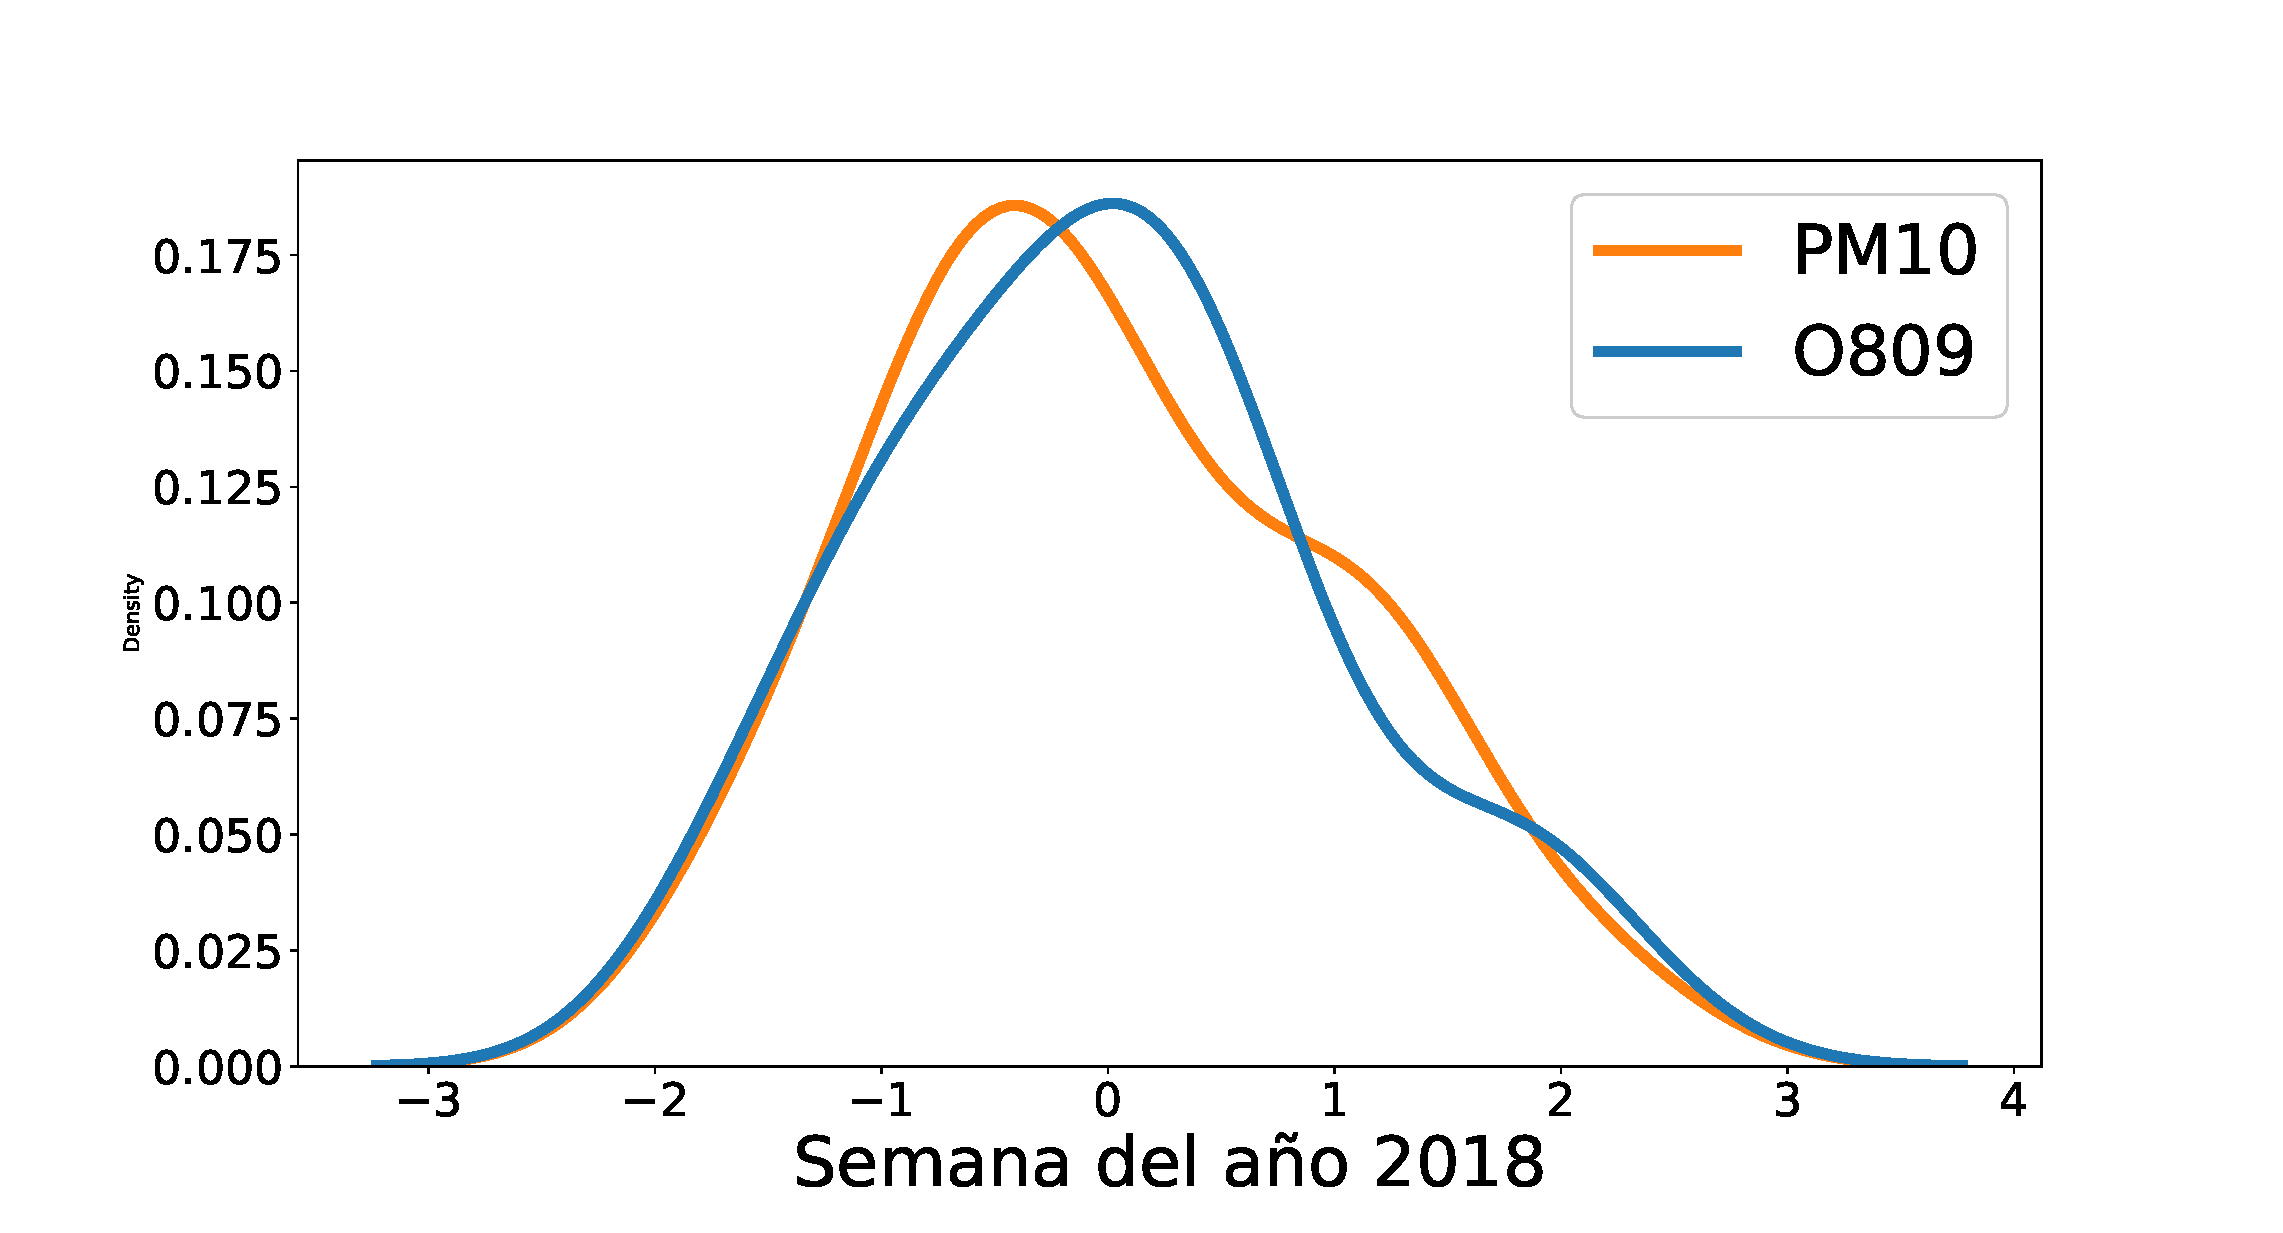
\includegraphics[width=1\textwidth]{PM10_O809_2018.eps}
%   \end{center}
%    \caption[Ejemplo de series de tiempo]{Evolución de los niveles de PM10 y el número de egresos diagnosticados con la CIE O809 en el 2018.}
%    \label{serie_de_tiempo}
%\end{figure}

\subsubsection{Gráficos de radar}
Los gráficos de radar o diagramas de telaraña son otra manera de visualizar un conjunto de datos. Sirven para comparar variables visualizando si existen valores o patrones de evolución en el tiempo similares entre ellas. Es por ello que en el presente trabajo se elaboran gráficos de radar con ayuda de \texttt{Python} y las librerías \texttt{NumPy} y \texttt{Matplotlib} \ref{tab:Herramientas utilizadas}. En la figura \ref{grafico_de_telaraña} se muestra un ejemplo de los gráficos de telaraña generados.

\begin{figure}[h!]
\setcounter{figure}{1} % por culpa de sciposter
\captionsetup{type=figure} % por culpa de sciposter
\begin{center}
   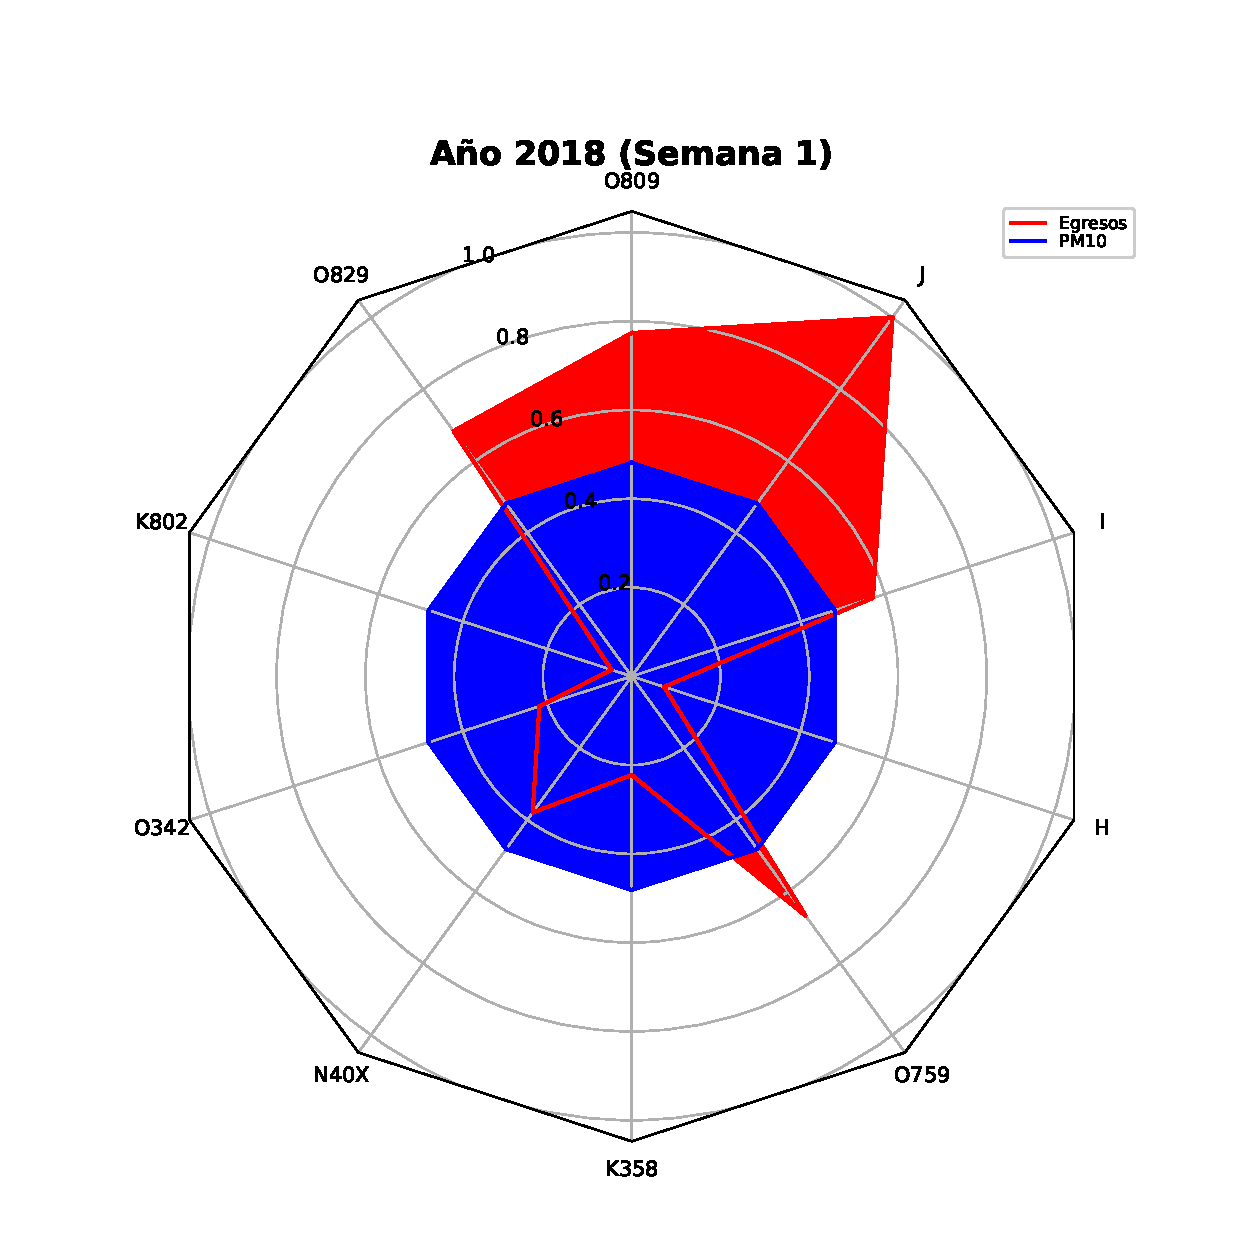
\includegraphics[width=1\textwidth]{spiderweb_PM10_2018_1.eps}
   \end{center}
    \caption[Ejemplo de gráfico de radar]{Nivel del contaminante PM10 y egresos por CIE en la semana 1 del año 2018.}
    \label{grafico_de_telaraña}
\end{figure}

\clearpage
\subsection{Implementación de modelos}
Después de haber generado gráficos para la visualización de la evolución de las variables, se procede a generar modelos para el estudio de la relación entre las variables. Para ello se utiliza \texttt{Python} y la librería \texttt{Statsmodels} \ref{tab:Herramientas utilizadas}. Los tipos de modelos generados se discuten a continuación.

\subsubsection{Regresión lineal}
Primeramente se calcula el coeficiente de correlación de Pearson, si el valor de la correlación se encuentre entre -1 y 1 significa que existe una dependencia lineal y que existe sustento para el modelo de regresión lineal. El modelo de regresión lineal arroja un valor de $R^2$ que indica en que grado la variable independiente explica la varianza de la variable dependiente. Además, se obtiene el valor $p$ que indica la relevancia del resultado y se obtiene la raíz de error cuadrático medio (RMSE) que indica cuantas unidades se alejan los valores predichos por el modelo de los valores reales, eso ayuda a determinar el error del modelo.

\subsubsection{Regresión lineal múltiple}
En los modelos de regresión lineal múltiple se tiene más de una variable independiente. Al obtener el valor de la correlación entre -1 y 1 para verificar que existe sustento para el modelo de regresión lineal, se procede a generar el modelo de regresión lineal múltiple. El modelo de regresión lineal múltiple arroja un valor de $R^2$ que indica en que grado las variables independientes explican la varianza de la variable dependiente. Además, se obtiene el valor $p$ que indica la relevancia del resultado y se obtiene la raíz de error cuadrático medio (RMSE) que indica cuantas unidades se alejan los valores predichos por el modelo de los valores reales, eso ayuda a determinar el error del modelo.

\section{Implementación de la solución propuesta}
% Recapitulando las fases anteriores, se conoce que...
En implementación de la solución propuesta se muestra el desarrollo realizado de los puntos planteados en \ref{Diseño de la solución propuesta}. El desarrollo del presente proyecto se encuentra en el siguiente repositorio Github: \url{https://github.com/selenebpradop/relaciones-contaminantes-salud/}.

\begin{description}
\item{En la función \ref{lst:c1} se muestra el proceso realizado para el procesamiento y agrupamiento de los datos en semanas epidemiológicas.}
\item{El fragmento de código \ref{lst:c2} muestra como es que se generan las series de tiempo, esto después de haber procesado y agrupado los datos.}
\item{La función mostrada en \ref{lst:c3} genera gráficos de radar al ingresarle como parámetros los datos ya procesados y agrupados.}
\item{En el fragmento de código \ref{lst:c4} se muestra como son generados los modelos de regresión lineal después de haber procesado y agrupado los datos.}
\end{description}

\clearpage

\begin{lstlisting}[language=Python, caption=Procesamiento y agrupamiento de datos, label=lst:c1]
import pandas as pd
from epiweeks import Week, date
from sklearn import preprocessing
import seaborn as sns
import matplotlib.pyplot as plt
import string

columns = ['timestamp', contaminante]
dataframec = pd.read_csv('filled.csv', usecols=columns).dropna()
strfdt = '%d-%b-%y %H'
dataframec['timestamp'] = pd.to_datetime(dataframec['timestamp'], errors = 'coerce', format=strfdt)
dataframec = dataframec.dropna()
dataframec = dataframec.reset_index(drop=True)
dataframec['timestamp'] = dataframec['timestamp'].apply(lambda x: x.strftime('%Y-%m-%d %H'))
dataframeca = dataframec.loc[dataframec['timestamp'].str.startswith(año)]
dataframeca = dataframeca.reset_index(drop=True)
strfdt = '%Y-%m-%d %H'
dataframeca['timestamp'] = pd.to_datetime(dataframeca['timestamp'], errors = 'coerce', format=strfdt)
dataframeca['sem'] = dataframeca['timestamp'].apply(lambda x: date(x.year, x.month, x.day))
dataframeca['sem'] = dataframeca['sem'].apply(lambda x: Week.fromdate(x))
dataframeca['sem'] = dataframeca['sem'].apply(lambda x: x.week)
colums = ['EGRESO', 'DIAG_INI']
csvegresos = 'EGRESO_' + año + '.csv'
dataframeea = pd.read_csv(csvegresos, usecols=colums).dropna()
dataframeea['EGRESO'] = pd.to_datetime(dataframeea['EGRESO'], errors = 'coerce', format=strfdto)
dataframeea = dataframeea.loc[dataframeea['ENTIDAD'] == entidad]
dataframeea = dataframeea.dropna()
dataframeea = dataframeea.reset_index(drop=True)
numaño = int(año) 
dataframeea['sem'] = dataframeea['EGRESO'].apply(lambda x: date(x.year, x.month, x.day))
dataframeea['sem'] = dataframeea['sem'].apply(lambda x: Week.fromdate(x))
dataframeea['sem'] = dataframeea['sem'].apply(lambda x: x.week)
dataframeea['EGRESO'] = dataframeea['EGRESO'].apply(lambda x: x if(x.year==numaño) else pd.NaT)   
dataframeea = dataframeea.dropna()
dataframeea = dataframeea.reset_index(drop=True)
dataframesca = pd.DataFrame()
dataframesca['sem'] = semanas.index
dataframesca[contaminante] = ''
n = len(semanas.index)
for i in range (n):
    registrossem = dataframeca.loc[dataframeca['sem'] == i+1]
    promediocas = registrossem[contaminante].mean()
    dataframesca[contaminante][i] = promediocas
\end{lstlisting}

\begin{lstlisting}[language=Python, caption=Generación de series de tiempo, label=lst:c2]
import pandas as pd
from epiweeks import Week, date
from sklearn import preprocessing
import seaborn as sns
import matplotlib.pyplot as plt
import string

diagnosticosaño = dataframeea['DIAG_INI'].value_counts()
diagnosticosaño = diagnosticosaño.sort_values(ascending = False)
ciesaño = dataframeea.groupby(['DIAG_INI', 'sem']).count()

s_scaler = preprocessing.StandardScaler()
ind = []
n = len(semanas.index)
for i in range (n):
    ind.append(i+1)
letras = []
for letra in string.ascii_uppercase:
    letras.append(str(letra))
# Se inicia un contador para controlar la cantidad de graficos a generar
cont = 0
maximo = 10
mindividuales = 7

# Proceso de generación de las figuras
print('\n' + año)
for name in diagnosticosaño.index:
    if cont < maximo:
        dataframegraficoacc = pd.DataFrame()
        dataframegraficoacc[contaminante] = dataframesca[contaminante]
        dataframegraficoacc = dataframegacc.reindex(ind)
        if cont < mindividuales:
            dataframegacc[name] = ciesaño['EGRESO'][name]
            for i in range (n):
                dataframegacc[contaminante][i+1] = dataframesca[contaminante][i]
            col_names = [contaminante, name]    
        else:
            nameg =  letras[cont]
            ciesagrupadas = dataframeea.loc[dataframeea['DIAG_INI'].str.startswith(nameg)]
            ciesagrupadas = ciesagrupadas['sem'].value_counts()
            dataframegacc[nameg] = ciesagrupadas
            for i in range (n):
                dataframegacc[contaminante][i+1] = dataframesca[contaminante][i]
            col_names = [contaminante, nameg]
        df_s = s_scaler.fit_transform(dataframegacc)
        df_s = pd.DataFrame(df_s, columns=col_names)
        fig, ax = plt.subplots(ncols=1, figsize=(20, 8))
        print('\n' + col_names[0] + ' & ' + col_names[1])
        ax.set_title('Contaminante ' + col_names[0] + ' & CIE ' + col_names[1])
        ax.set_xlabel('Semana del año ' + año)
        sns.kdeplot(data=df_s)
        plt.savefig(contaminante + '/' + col_names[0] + '&' + col_names[1] + '_' + año + '.jpg', format='jpg')
        plt.show()
    cont = cont+1
\end{lstlisting}

\begin{lstlisting}[language=Python, caption=Generación de graficos de radar, label=lst:c3]
def create_spiderwebs(datasets, lenlines, numspiders, title, titles, spoke_labels, colors, typeframe):

    # Set the number of lines of each spiderweb
    N = len(datasets)
    theta = radar_factory(N, frame=typeframe)
    # Set the number of columns and rows
    if (numspiders%2==0):
        numrows = 2
        numcols = int(numspiders/2)
    else:
        numrows = 1
        numcols = numspiders
        
    # Draw the shape of the spiderweb
    fig, axs = plt.subplots(figsize=(8, 8), nrows=numrows, ncols=numcols, subplot_kw=dict(projection='radar'))
    fig.subplots_adjust(wspace=0.5, hspace=0.20, top=0.85, bottom=0.05)
    newn = 0.5
    rgrids = []
    for z in range(lenlines*2):
        rgrids.append(newn)
        newn = newn + 0.5

    # Counter of the number of spiders
    i=0

    # Plot each case on separate axes
    for ax, (titlespiderweb) in zip(axs.flat, titles):
        # Put labels in the lines
        ax.set_rgrids(rgrids)        
        ax.set_title(titlespiderweb, weight='bold', size='medium', position=(0.5, 1.1))
        dataspider = []
        # Normalize data
        for y in range(N):
            currentdata = datasets[y]
            number = currentdata[i]
            nmin = min(currentdata);
            nmax = max(currentdata);
            r = nmax - nmin
            x = (number-nmin)/r
            y = lenlines*x
            dataspider.append(y)
        # Draw the new lines in the spiderweb
        ax.plot(theta, dataspider, color=colors[i])
        ax.fill(theta, dataspider, facecolor=colors[i], alpha=0.25)
        # Put the name of each line in the figure
        ax.set_varlabels(spoke_labels)
        # Increment the counter
        i=i+1
    # Show the figure
    plt.show()
\end{lstlisting}

\begin{lstlisting}[language=Python, caption=Generación de los modelos de regresión lineal, label=lst:c4]
datos = pd.DataFrame(dataframegacc, columns=col_names)
# Gráfico
# ==============================================================================
fig, ax = plt.subplots(figsize=(6, 3.84))
datos.plot(
    x    = col_names[0],
    y    = col_names[1],
    c    = 'firebrick',
    kind = "scatter",
    ax   = ax
)
ax.set_title('Contaminante ' + col_names[0] + ' & CIE ' + col_names[1])

# Correlación lineal entre las dos variables
# ==============================================================================
corr_test = pearsonr(x = datos[col_names[0]].fillna(0), y =  datos[col_names[1]].fillna(0))
print("Coeficiente de correlación de Pearson: ", corr_test[0])
print("P-value: ", corr_test[1])

# División de los datos en train y test
# ==============================================================================
xx = datos[[col_names[0]]].fillna(0)
yy = datos[[col_names[1]]].fillna(0)
        
x2 = xx.values.tolist()
y2 = yy.values.tolist()

# Creación del modelo utilizando matrices como en scikitlearn
# ==============================================================================
# A la matriz de predictores se le tiene que añadir una columna de 1s para el intercept del modelo
x = np.array(x2).astype(float)
y = np.array(y2).astype(float)
#ones = np.ones(len(x[0]))
#X = sm.add_constant(np.column_stack((x[0], ones)))
#for ele in x[1:]:
#    X = sm.add_constant(np.column_stack((ele, X)))
modelo = sm.OLS(y, x)
modelo = modelo.fit()
print(modelo.summary())
\end{lstlisting}

\chapter{Experimentos}

En el presente capítulo se presenta el diseño de los experimentos realizados así como los resultados obtenidos de ellos.

En esta sección se tratan los resultados obtenidos partiendo de desarrollar algunos experimentos que permiten determinar si la solución propuesta cumple con el objetivo planteado.

\section{Diseño experimental}
En la presente sección se discute el diseño de experimentos, es decir, qué valores constantes fueron utilizados para su realización y por qué se usan dichos valores.

\subsection{Datos de entrada}
Los datos de egresos hospitalarios de los años 2017 y 2018 provienen de la base de datos de la Secretaría de Salud del Gobierno de México \cite{f1}. También se tienen registros de los niveles de PM10 y PM2.5 presentes en el área metropolitana de Monterrey, dichos registros son obtenidos por las estaciones de monitoreo pertenecientes al SIMA \cite{f2} mostradas en la figura \ref{estaciones} en la página \pageref{estaciones}. Los documentos con los datos son proporcionados por \citet{f3}.

\begin{description}
\item [Selección de datos.] {Los conjuntos de datos por año de egresos hospitalarios contienen información de todos los estados de México, por lo cual se hace una limpieza de datos para solo obtener los registros de Nuevo León ya que de dicha entidad es de la cual se tienen los datos de contaminación.}
\item [Datos de ingresos hospitalarios.] {Se agrupan en semanas epidemiológicas para una mejor manipulación de ellos. Por CIE se obtiene el número de egresos en cada semana del año ordenadas por el número de egresos en el año partiendo de la CIE con la mayor cantidad.}
\item [Datos de los contaminantes.] {Se agrupan en semanas epidemiológicas para una mejor manipulación de ellos. Se obtiene el promedio del nivel del contaminante por cada semana del año.}
\end{description}

\subsection{Visualización de datos}
Con los datos ya seleccionados y agrupados se procede a generar las visualizaciones de los datos. Las visualizaciones de los datos se hacen con series de tiempo y gráficos de radar.

\begin{description}
\item [Series de tiempo.] {Se procede a generar series de tiempo de cada año por contaminante y CIE}. Las variables ajustables son:
\begin{itemize}
	\item El nombre del contaminante.
	\item El año del que se quieren obtener las series de tiempo.
	\item Número de series de tiempo a generar por contaminante. Se parte de la CIE con mayor número de egresos.
\end{itemize}

\item [Gráficos de radar.] {Los datos ya seleccionados y agrupados se normalizan teniendo como valor mínimo cero y como valor máximo un número entre uno y cuatro. Posteriormente se generan gráficos de radar de cada año por semana, en las que se muestra el nivel contaminante y la variación de las CIE}. Las variables ajustables son:
\begin{itemize}
    \item Cantidad de CIE a agregar en el gráfico. Se parte de la CIE con mayor número de egresos.
	\item Valor máximo que se utiliza para representar la longitud de los ejes en el gráfico.
	\item Nombre de la figura.
	\item Nombre de cada eje en el gráfico.
	\item Los colores de cada eje en el gráfico. 
	\item Si el gráfico es generado de forma circular o en forma de polígono.
\end{itemize}
\end{description}

\subsection{Generación de modelos}
Se procede a generar los modelos. En cada modelo se tienen métricas para evaluar su eficacia y valores que pueden ser ajustados en función de encontrar la combinación que proporcione mejores resultados.

Se tienen algunas variables que pueden ser modificadas para la generación de los modelos de regresión lineal.

\begin{itemize}
	\item Cantidad de CIE a agregar en el modelo. Se parte de la CIE con mayor número de egresos.
	\item Porcentaje de datos utilizados para el entrenamiento del modelo.
	\item Nivel de significancia.
\end{itemize}

También se tienen variables que indican información sobre la eficacia del modelo.

\begin{itemize}
	\item Valor $p$.
	\item $R^2$ (R cuadrado).
	\item Raíz de error cuadrático medio (RMSE).
\end{itemize}


\clearpage
\section{Resultados}
Establecidas las especificaciones de los experimentos que se realizan, se reportan los resultados obtenidos. Los experimentos se elaboran por contaminante, desglosando los resultados por año. En la carpeta \url{https://github.com/selenebpradop/relaciones-contaminantes-salud/tree/main/figuras/} se encuentran animaciones en video de los gráficos de radar generados por contaminante y año y todas las imágenes de las series de tiempo obtenidas.

% FORMULA PORCENTAJE ERROR
\subsection{Experimento A: Datos de niveles de PM10}
Se estudian los niveles del contaminante PM10 de los años 2017 y 2018. 

\subsubsection{Año 2017}
En la figura \ref{serie_de_tiempo_2017_PM10} se muestra una de las series de tiempo generadas para la CIE con mayor número de egresos registrados en el conjunto de datos del año. Además, en el cuadro \ref{tab:Resultados obtenidos PM10 2017} se presentan los resultados obtenidos de los modelos de regresión lineal y la eficacia obtenida de dichos modelos. El cuadro \ref{tab:RRLM PM10 2017} muestra los resultados del modelo de regresión lineal múltiple. En la figura \ref{correlaciones_2017_PM10} se muestran las correlaciones obtenidas en un gráfico de radar.

\begin{figure}[h!]
\setcounter{figure}{0} % por culpa de sciposter
\captionsetup{type=figure} % por culpa de sciposter
\begin{center}
   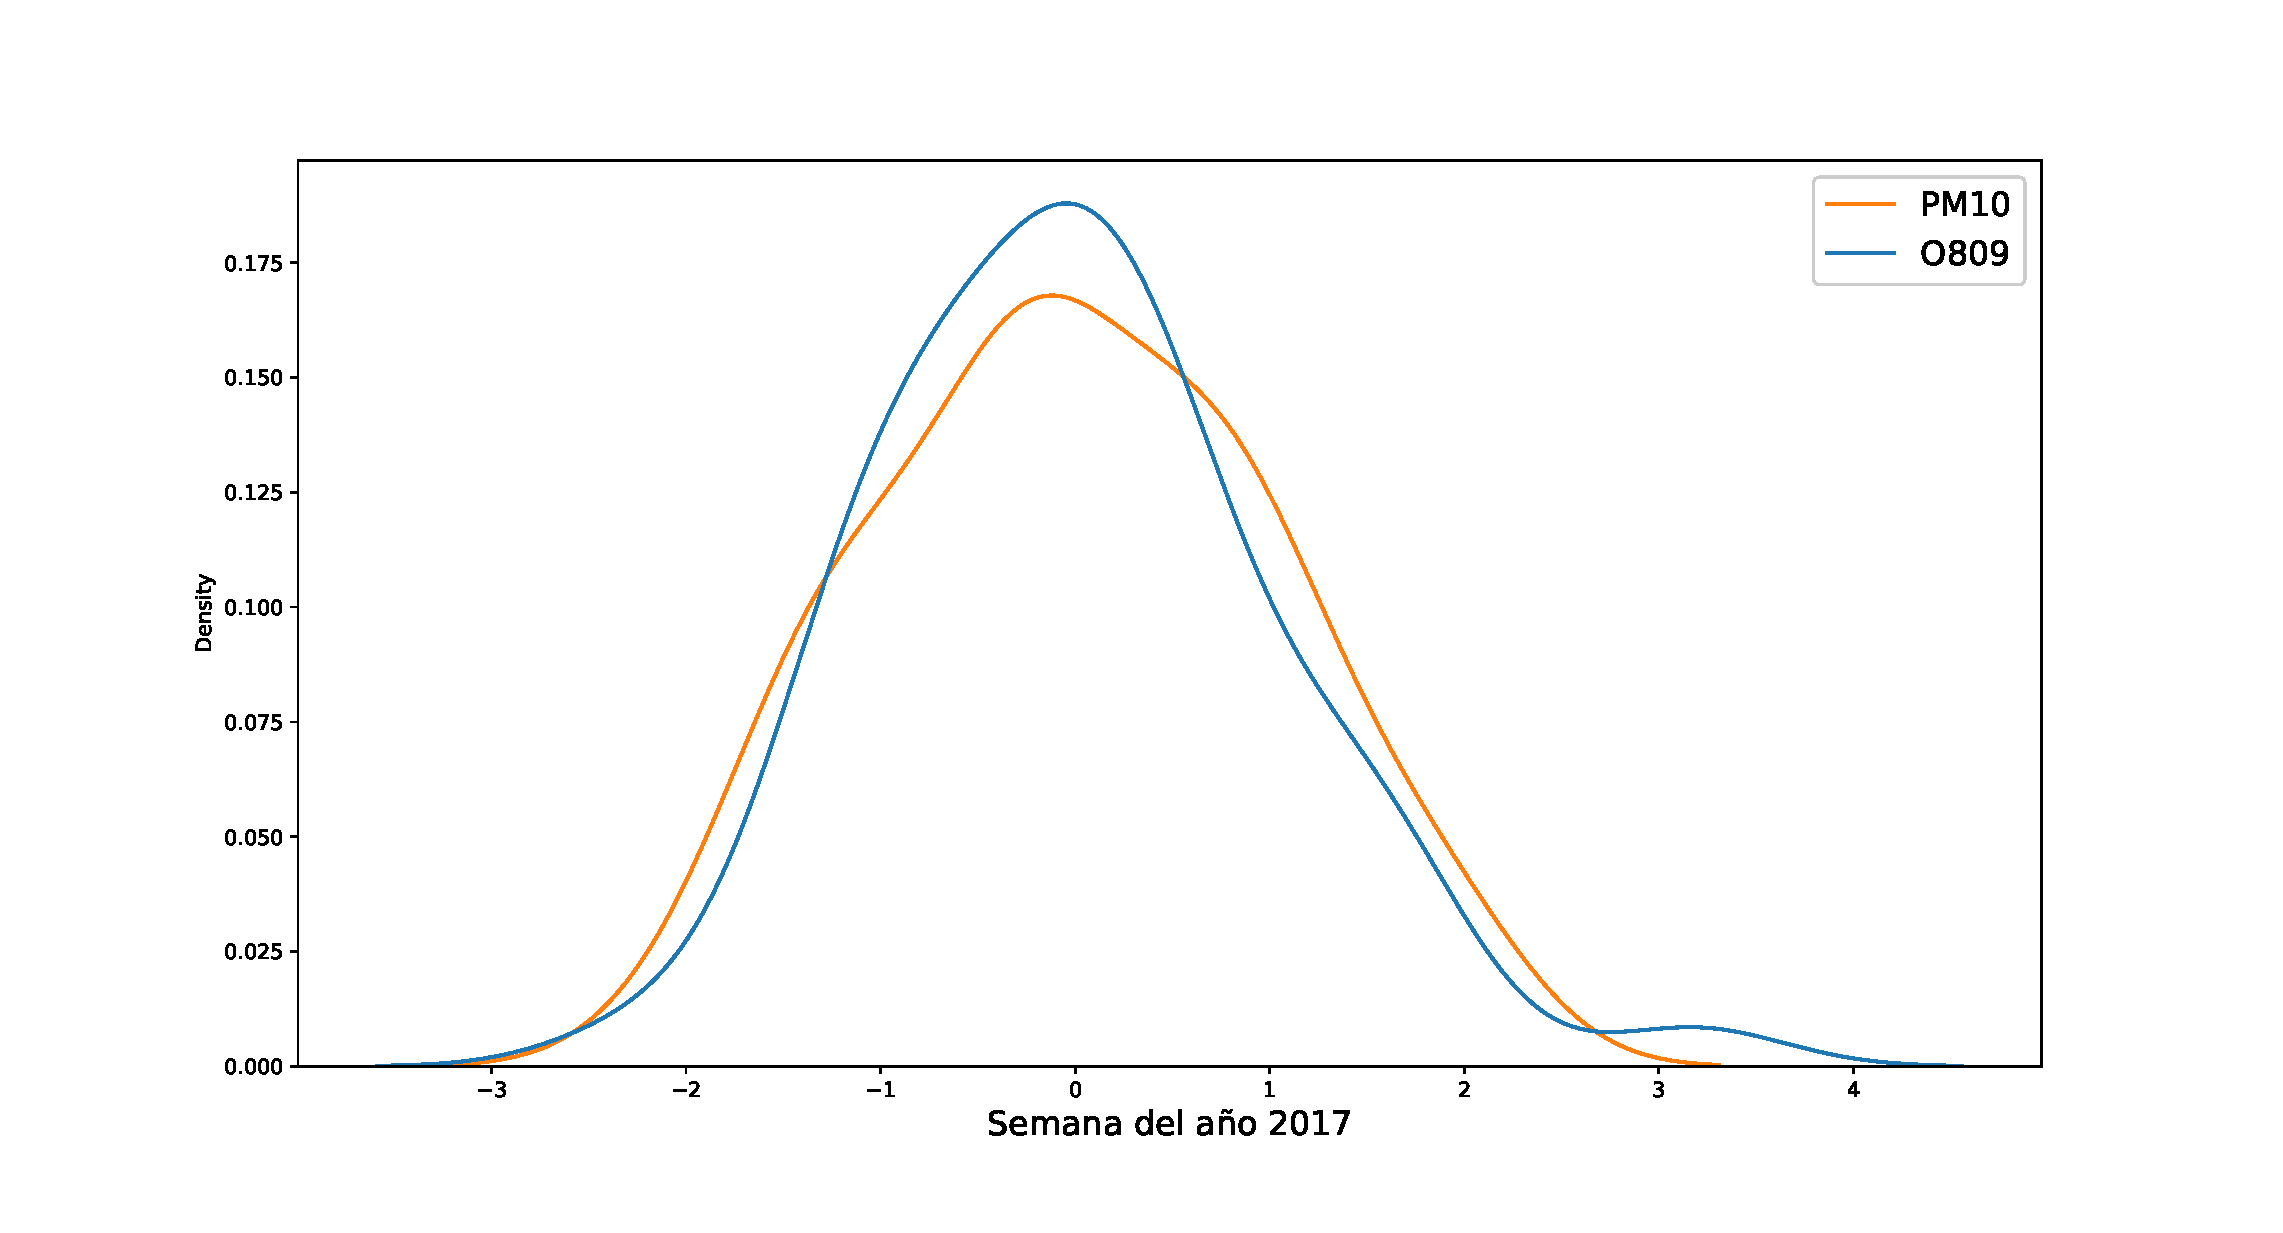
\includegraphics[trim=61 0 0 0,clip,width=1\textwidth]{PM10_O809_2017.eps}
   \end{center}
    \caption[Series de tiempo 2017 PM10 y O809]{Evolución de los niveles de PM10 y el número de egresos diagnosticados con la CIE O809 en el 2017.}
    \label{serie_de_tiempo_2017_PM10}
\end{figure}

\begin{table}[hbt!]
\centering
\caption{Resultados obtenidos PM10 2017}
\label{tab:Resultados obtenidos PM10 2017}
\vspace{0.5cm}
\begin{threeparttable}
\begin{tabular}{|c|c|c|c|c|}
	\hline
	CIE & $\rho$ & $R^2$ & Valor $p$ & $\epsilon$\\
	\hline
	O809 & -0.275 & 0.061 & 0.121 & 0.239 \\
	\hline
	O829 & 0.100 & 0.091 & 0.055 & 0.287 \\
	\hline
	O759 & -0.085 & 0.116 & 0.029 & 0.294 \\
	\hline
	O069 & -0.247 & 0.070 & 0.094 & 0.222 \\
	\hline
	K802 & 0.044 & 0.005 & 0.658 & 0.282 \\
	\hline
\end{tabular}
\begin{tablenotes}
\footnotesize
\item{$\rho$ = Coeficiente de correlación de Pearson}
\item{$\epsilon$ = RMSE para medir el error}
\end{tablenotes}
\end{threeparttable}
\end{table}

\begin{figure}[h!]
\setcounter{figure}{1} % por culpa de sciposter
\captionsetup{type=figure} % por culpa de sciposter
\begin{center}
   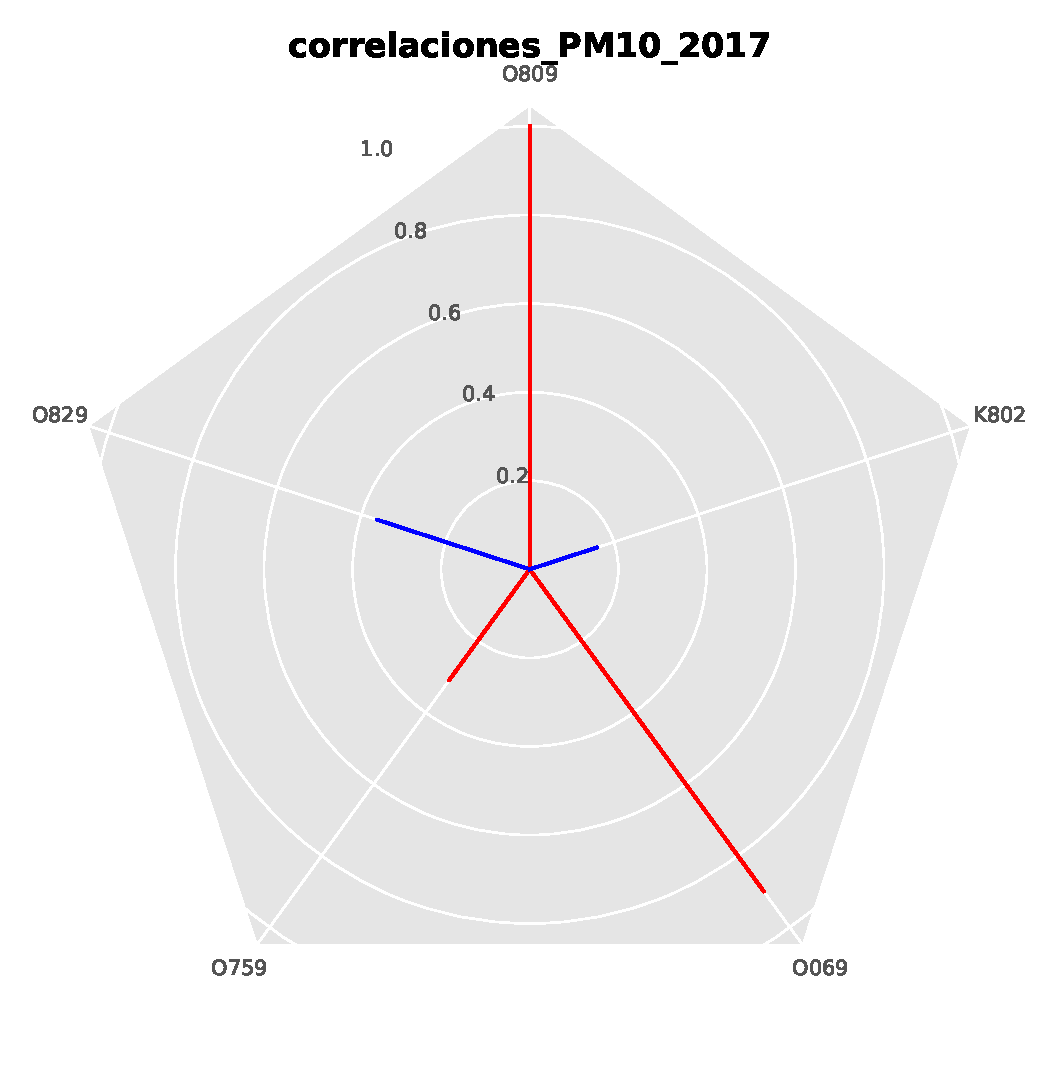
\includegraphics[trim=0 0 0 23,clip,width=1\textwidth]{spiderweb_correlaciones_PM10_2017}
   \end{center}
    \caption[Correlaciones 2017 PM10]{Correlaciones entre los niveles de PM10 y CIE en el 2017 donde el azul indica una correlación positiva y el rojo una correlación negativa.}
    \label{correlaciones_2017_PM10}
\end{figure}

\begin{table}[hbt!]
\caption{Resultados regresión lineal múltiple PM10 2017}
\label{tab:RRLM PM10 2017}
\begin{center}
\begin{tabular}{lclc}
\toprule
\textbf{Variable Dep.:}    &        $y$         & \textbf{  R$^2$:         } &     0.313   \\
\textbf{Modelo:}            &       OLS        & \textbf{Método:}           &  Mínimos cuadrados  \\
\textbf{Error:}            & 0.226  \\
\bottomrule
\end{tabular}
\begin{tabular}{lcccccc}
               & \textbf{coef} & \textbf{std err} & \textbf{$t$} & \textbf{P$> |$t$|$} & \textbf{[0.025} & \textbf{0.975]}  \\
\midrule
\textbf{const} &       0.5859  &        0.146     &     4.002  &         0.000        &        0.289    &        0.883     \\
\textbf{O809}  &      -0.3019  &        0.122     &    -2.472  &         0.018        &       -0.550    &       -0.054     \\
\textbf{O829}  &       0.2685  &        0.123     &     2.185  &         0.036        &        0.019    &        0.518     \\
\textbf{O759}  &      -0.2229  &        0.182     &    -1.222  &         0.230        &       -0.593    &        0.147     \\
\textbf{O069}  &      -0.1441  &        0.120     &    -1.200  &         0.238        &       -0.388    &        0.100     \\
\textbf{K802}  &      -0.0456  &        0.133     &    -0.344  &         0.733        &       -0.315    &        0.224     \\
\bottomrule
\end{tabular}
\end{center}
\end{table}

\clearpage
\subsubsection{Año 2018}
En la figura \ref{serie_de_tiempo_2018_PM10} se muestra una de las series de tiempo generadas para la CIE con mayor número de egresos registrados en el conjunto de datos del año. Además, en el cuadro \ref{tab:Resultados obtenidos PM10 2018} se presentan los resultados obtenidos de los modelos de regresión lineal y la eficacia obtenida de dichos modelos. El cuadro \ref{tab:RRLM PM10 2018} muestra los resultados del modelo de regresión lineal múltiple. En la figura \ref{correlaciones_2018_PM10} se muestran las correlaciones obtenidas en un gráfico de radar.

\begin{figure}[h!]
\setcounter{figure}{2} % por culpa de sciposter
\captionsetup{type=figure} % por culpa de sciposter
\begin{center}
   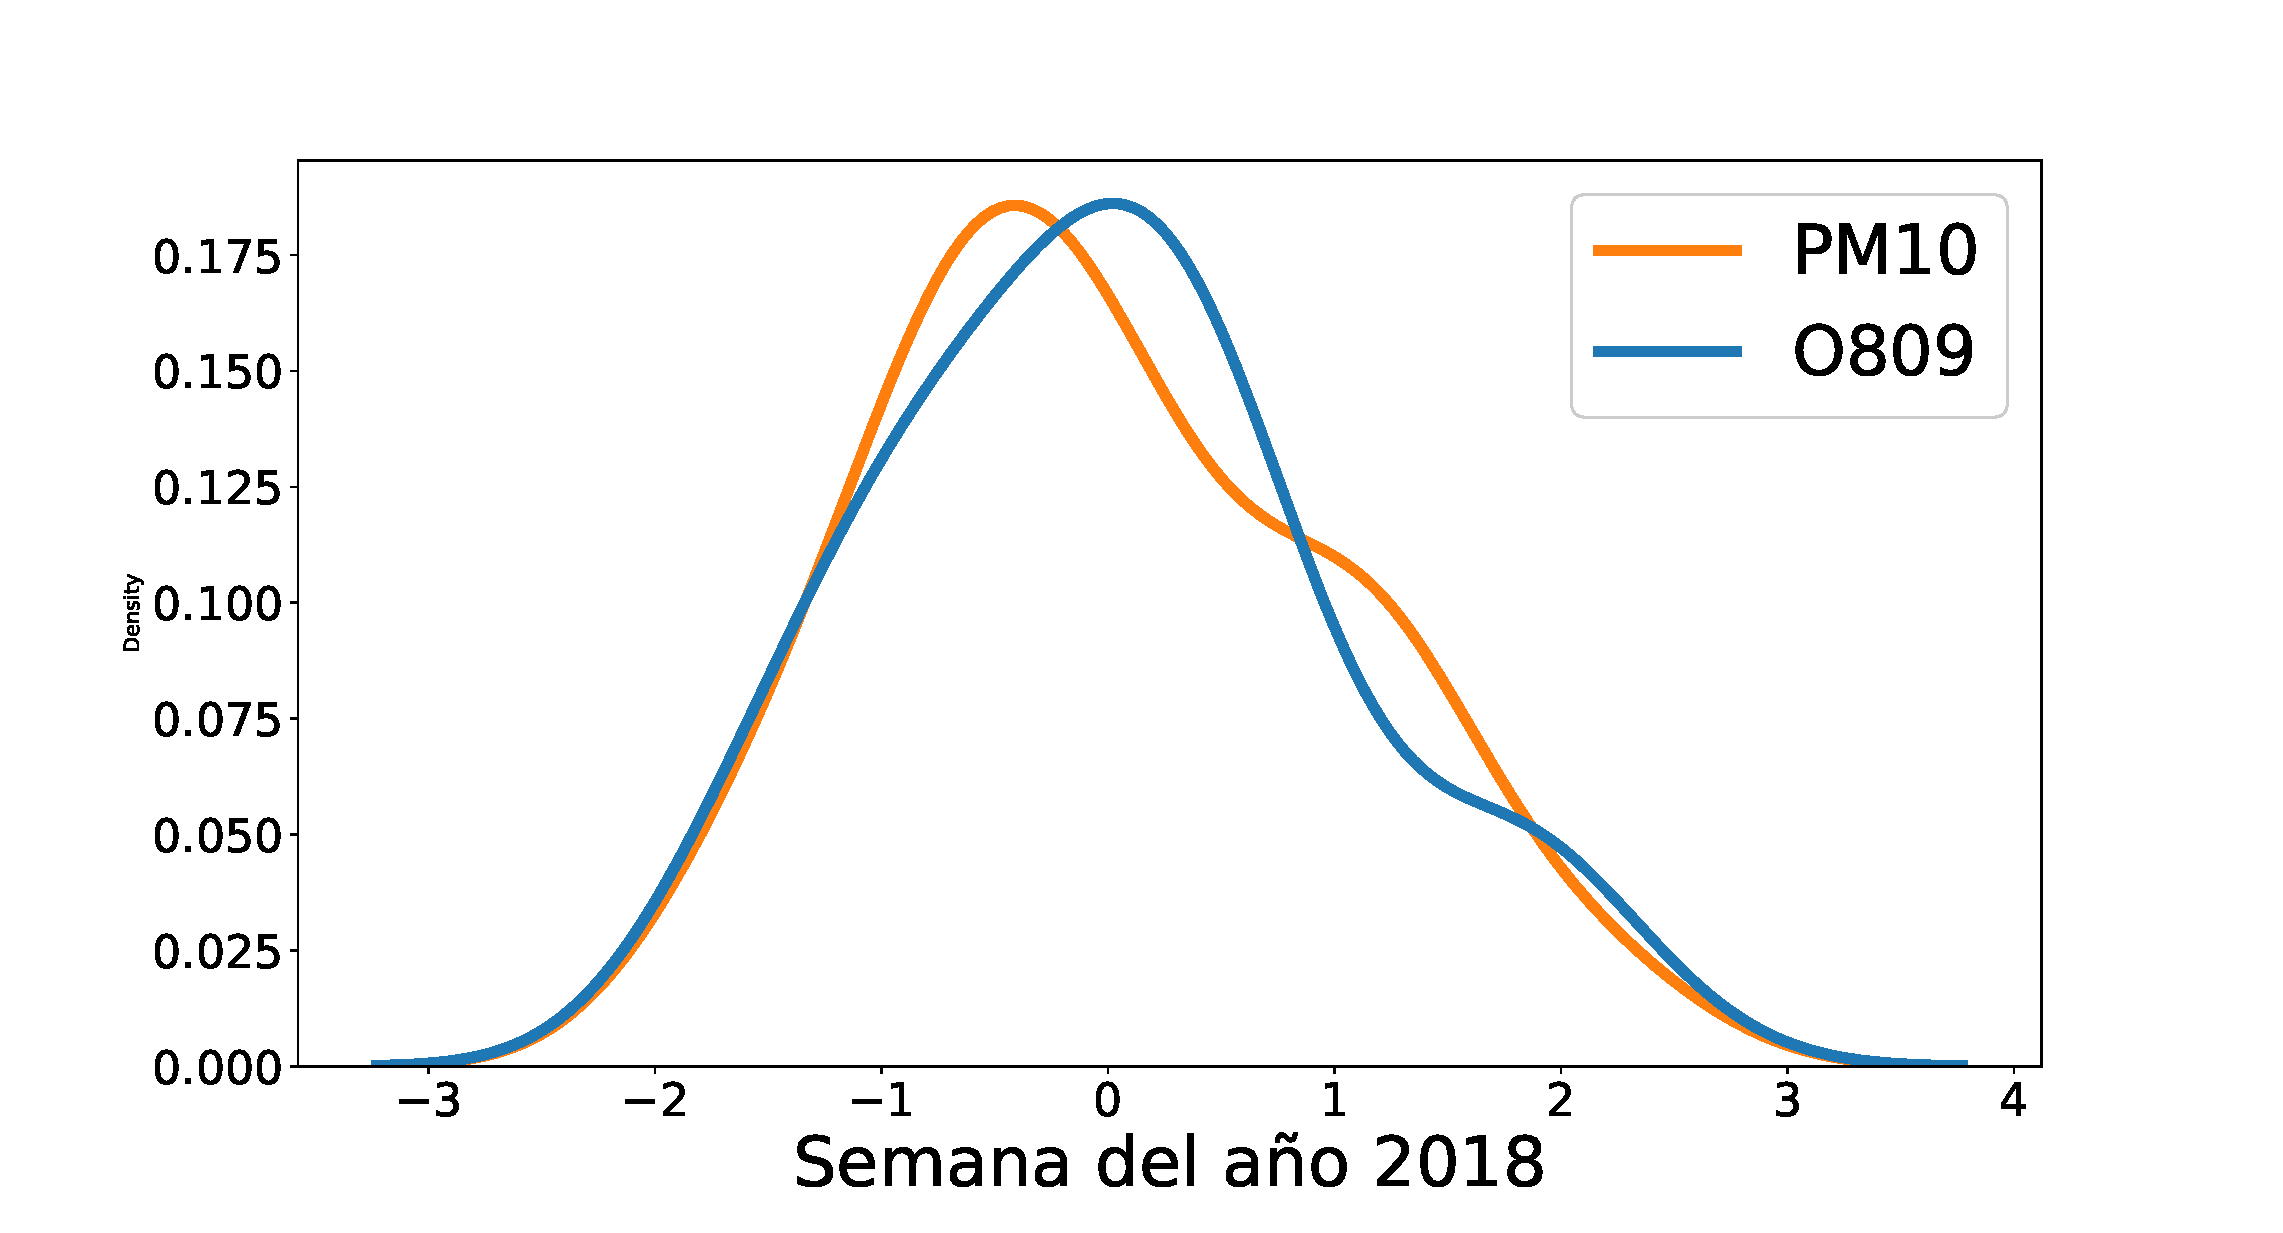
\includegraphics[trim=61 0 0 0,clip,width=1\textwidth]{PM10_O809_2018.eps}
   \end{center}
    \caption[Series de tiempo 2018 PM10 y O809]{Evolución de los niveles de PM10 y el número de egresos diagnosticados con la CIE O809 en el 2018.}
    \label{serie_de_tiempo_2018_PM10}
\end{figure}

\begin{table}[hbt!]
\centering
\caption{Resultados obtenidos PM10 2018}
\label{tab:Resultados obtenidos PM10 2018}
\vspace{0.5cm}
\begin{threeparttable}
\begin{tabular}{|c|c|c|c|c|}
	\hline
	CIE & $\rho$ & $R^2$ & Valor $p$ & $\epsilon$\\
	\hline
	O809 & -0.271 & 0.015 & 0.440 & 0.275 \\
	\hline
	O829 & 0.282 & 0.069 & 0.098 & 0.249 \\
	\hline
	K802 & 0.277 & 0.084 & 0.066 & 0.152 \\
	\hline
	O342 & -0.401 & 0.100 & 0.044 & 0.248 \\
	\hline
	N40X & -0.009 & 0.000 & 0.964 & 0.243 \\
	\hline
\end{tabular}
\begin{tablenotes}
\footnotesize
\item{$\rho$ = Coeficiente de correlación de Pearson}
\item{$\epsilon$ = RMSE para medir el error}
\end{tablenotes}
\end{threeparttable}
\end{table}

\begin{figure}[h!]
\setcounter{figure}{3} % por culpa de sciposter
\captionsetup{type=figure} % por culpa de sciposter
\begin{center}
   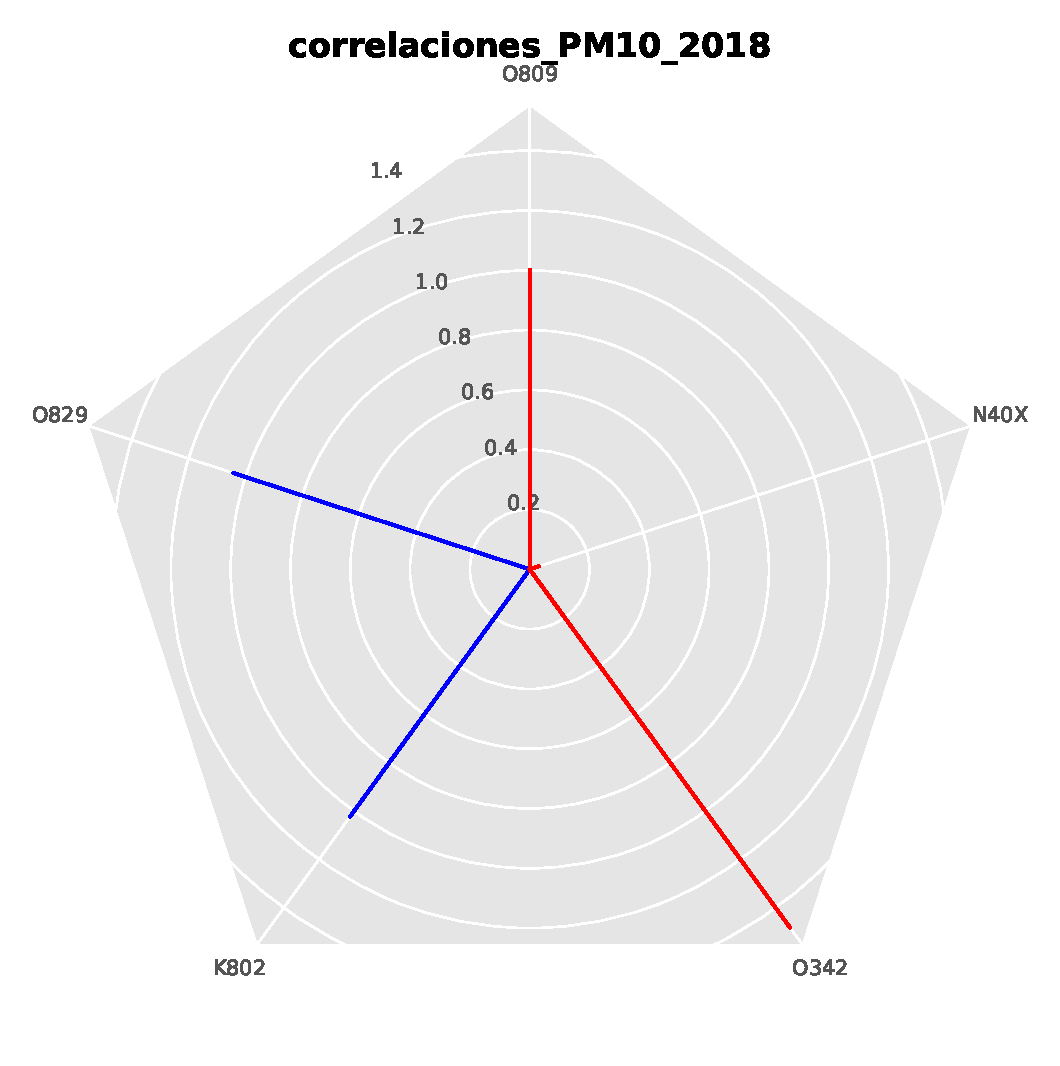
\includegraphics[trim=0 0 0 23,clip,width=1\textwidth]{spiderweb_correlaciones_PM10_2018}
   \end{center}
    \caption[Correlaciones 2018 PM10]{Correlaciones entre los niveles de PM10 y CIE en el 2018 donde el azul indica una correlación positiva y el rojo una correlación negativa.}
    \label{correlaciones_2018_PM10}
\end{figure}

\begin{table}[hbt!]
\caption{Resultados regresión lineal múltiple PM10 2018}
\label{tab:RRLM PM10 2018}
\begin{center}
\begin{tabular}{lclc}
\toprule
\textbf{Variable Dep.:}    &        $y$         & \textbf{  R$^2$:         } &     0.182   \\
\textbf{Modelo:}            &       OLS        & \textbf{Método:}           &  Mínimos cuadrados  \\
\textbf{Error:}            & 0.159  \\
\bottomrule
\end{tabular}
\begin{tabular}{lcccccc}
               & \textbf{coef} & \textbf{std err} & \textbf{$t$} & \textbf{P$> |$t$|$} & \textbf{[0.025} & \textbf{0.975]}  \\
\midrule
\textbf{const} &       0.3885  &        0.210     &     1.849  &         0.073        &       -0.038    &        0.815     \\
\textbf{O809}  &      -0.0114  &        0.188     &    -0.061  &         0.952        &       -0.392    &        0.370     \\
\textbf{O829}  &       0.0854  &        0.214     &     0.400  &         0.692        &       -0.349    &        0.520     \\
\textbf{K802}  &       0.3088  &        0.167     &     1.852  &         0.072        &       -0.030    &        0.647     \\
\textbf{O342}  &      -0.1708  &        0.208     &    -0.820  &         0.418        &       -0.593    &        0.252     \\
\textbf{N40X}  &      -0.1239  &        0.167     &    -0.740  &         0.464        &       -0.464    &        0.216     \\
\bottomrule
\end{tabular}
\end{center}
\end{table}


\clearpage
\subsection{Experimento B: Niveles de PM2.5}
Se estudian los niveles del contaminante PM2.5 de los años 2017 y 2018.

\subsubsection{Año 2017}
En la figura \ref{serie_de_tiempo_2017_PM25} se muestra una de las series de tiempo generadas para la CIE con mayor número de egresos registrados en el conjunto de datos del año. Además, en el cuadro \ref{tab:Resultados obtenidos PM2.5 2017} se presentan los resultados obtenidos de los modelos de regresión lineal y la eficacia obtenida de dichos modelos. El cuadro \ref{tab:RRLM PM2.5 2017} muestra los resultados del modelo de regresión lineal múltiple. En la figura \ref{correlaciones_2017_PM25} se muestran las correlaciones obtenidas en un gráfico de radar.

\begin{figure}[h!]
\setcounter{figure}{4} % por culpa de sciposter
\captionsetup{type=figure} % por culpa de sciposter
\begin{center}
   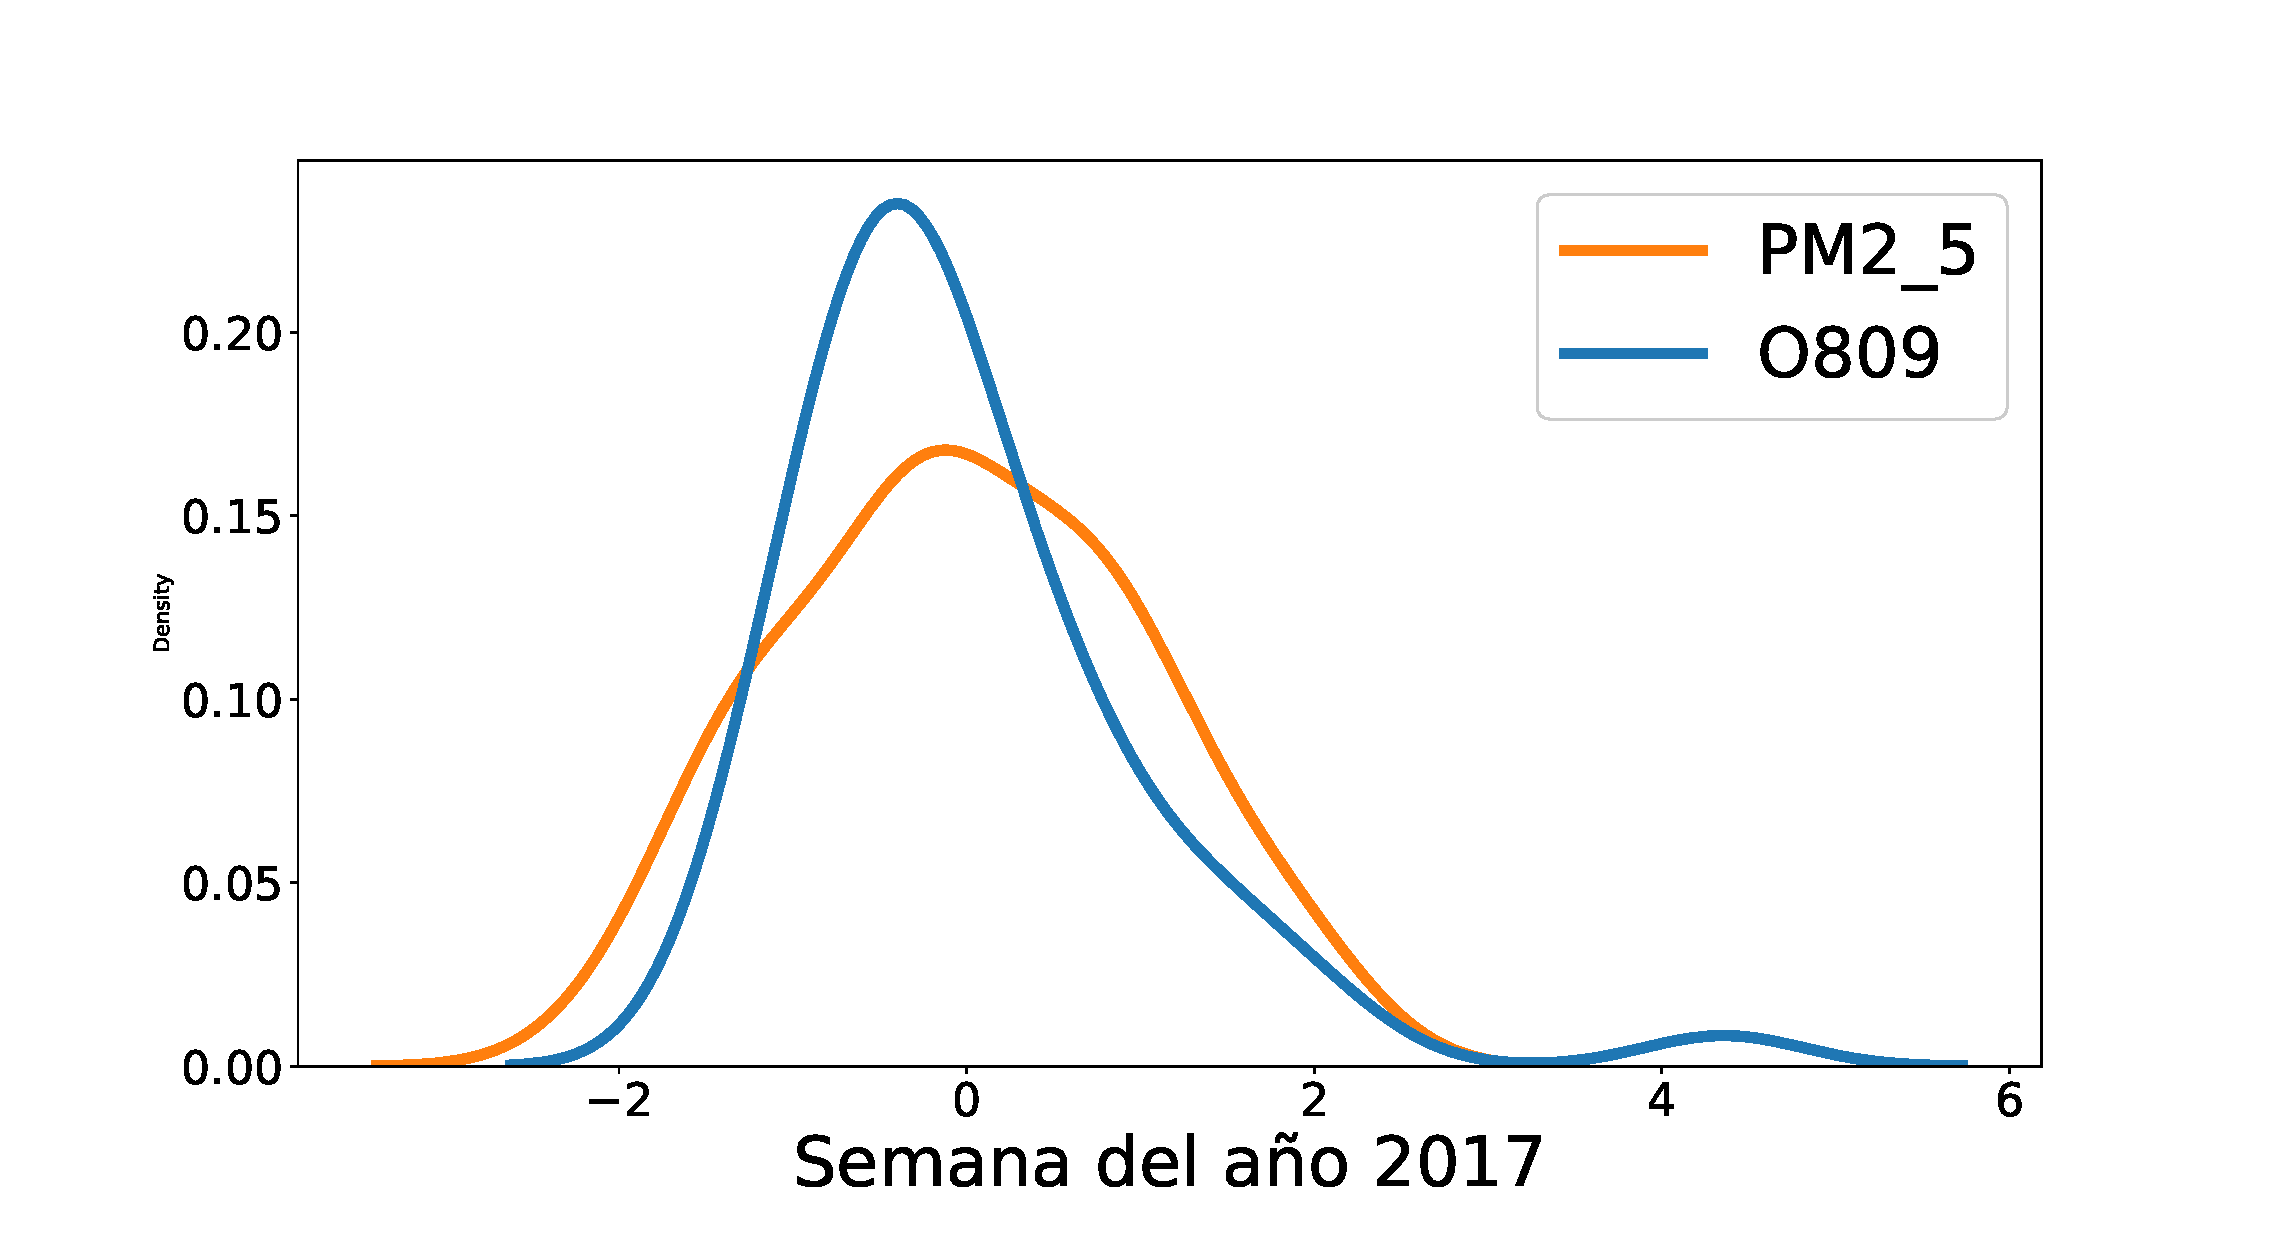
\includegraphics[trim=61 0 0 0,clip,width=1\textwidth]{PM2_5_O809_2017.eps}
   \end{center}
    \caption[Series de tiempo 2017 PM2.5 y O809]{Evolución de los niveles de PM2.5 y el número de egresos diagnosticados con la CIE O809 en el 2017.}
    \label{serie_de_tiempo_2017_PM25}
\end{figure}

\begin{table}[hbt!]
\centering
\caption{Resultados obtenidos PM2.5 2017}
\label{tab:Resultados obtenidos PM2.5 2017}
\vspace{0.5cm}
\begin{threeparttable}
\begin{tabular}{|c|c|c|c|c|}
	\hline
	CIE & $\rho$ & $R^2$ & Valor $p$ & $\epsilon$\\
	\hline
	O809 & -0.093 & 0.011 & 0.511 & 0.256 \\
	\hline
	O829 & 0.014 & 0.021 & 0.371 & 0.253 \\
	\hline
	O759 & -0.172 & 0.113 & 0.032 & 0.278 \\
	\hline
	O069 & -0.350 & 0.112 & 0.033 & 0.208 \\
	\hline
	K802 & 0.006 & 0.005 & 0.667 & 0.285 \\
	\hline
\end{tabular}
\begin{tablenotes}
\footnotesize
\item{$\rho$ = Coeficiente de correlación de Pearson}
\item{$\epsilon$ = RMSE para medir el error}
\end{tablenotes}
\end{threeparttable}
\end{table}

\begin{figure}[h!]
\setcounter{figure}{5} % por culpa de sciposter
\captionsetup{type=figure} % por culpa de sciposter
\begin{center}
   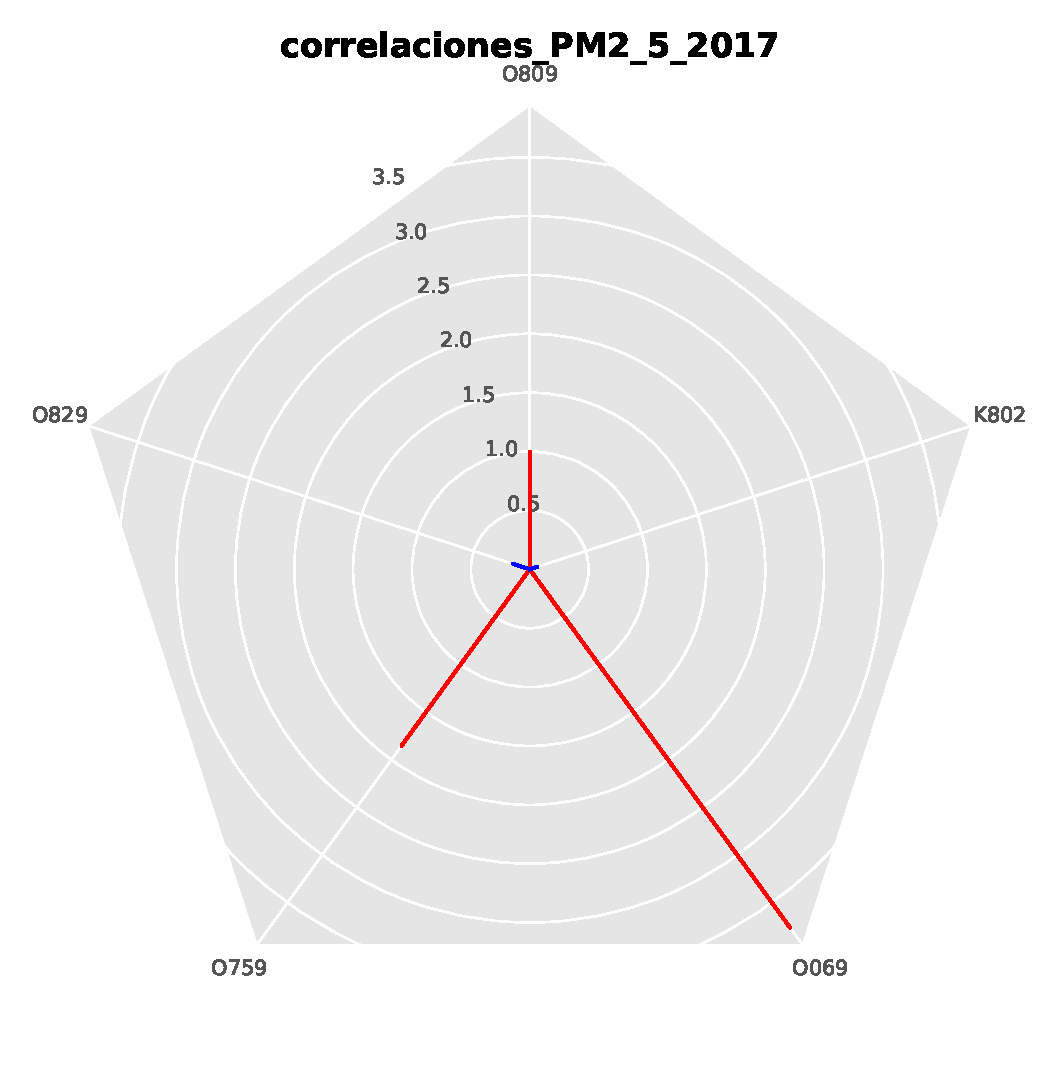
\includegraphics[trim=0 0 0 23,clip,width=1\textwidth]{spiderweb_correlaciones_PM2_5_2017}
   \end{center}
    \caption[Correlaciones 2017 PM2.5]{Correlaciones entre los niveles de PM2.5 y CIE en el 2017 donde el azul indica una correlación positiva y el rojo una correlación negativa.}
    \label{correlaciones_2017_PM25}
\end{figure}

\begin{table}[hbt!]
\caption{Resultados regresión lineal múltiple PM2.5 2017}
\label{tab:RRLM PM2.5 2017}
\begin{center}
\begin{tabular}{lclc}
\toprule
\textbf{Variable Dep.:}    &        $y$         & \textbf{  R$^2$:         } &     0.210   \\
\textbf{Modelo:}            &       OLS        & \textbf{Método:}           &  Mínimos cuadrados   \\
\textbf{Error:}            & 0.175  \\
\bottomrule
\end{tabular}
\begin{tabular}{lcccccc}
               & \textbf{coef} & \textbf{std err} & \textbf{$t$} & \textbf{P$> |$t$|$} & \textbf{[0.025} & \textbf{0.975]}  \\
\midrule
\textbf{const} &       0.5345  &        0.158     &     3.373  &         0.002        &        0.213    &        0.856     \\
\textbf{O809}  &      -0.1754  &        0.132     &    -1.327  &         0.193        &       -0.444    &        0.093     \\
\textbf{O829}  &       0.0701  &        0.133     &     0.527  &         0.602        &       -0.200    &        0.340     \\
\textbf{O759}  &      -0.2585  &        0.197     &    -1.309  &         0.199        &       -0.659    &        0.142     \\
\textbf{O069}  &      -0.2148  &        0.130     &    -1.652  &         0.108        &       -0.479    &        0.049     \\
\textbf{K802}  &      -0.1164  &        0.144     &    -0.811  &         0.423        &       -0.408    &        0.175     \\
\bottomrule
\end{tabular}
\end{center}
\end{table}

\clearpage
\subsubsection{Año 2018}
En la figura \ref{serie_de_tiempo_2018_PM25} se muestra una de las series de tiempo generadas para la CIE con mayor número de egresos registrados en el conjunto de datos del año. Además, en el cuadro \ref{tab:Resultados obtenidos PM2.5 2018} se presentan los resultados obtenidos de los modelos de regresión lineal y la eficacia obtenida de dichos modelos. El cuadro \ref{tab:RRLM PM2.5 2018} muestra los resultados del modelo de regresión lineal múltiple. En la figura \ref{correlaciones_2018_PM25} se muestran las correlaciones obtenidas en un gráfico de radar.

\begin{figure}[h!]
\setcounter{figure}{6} % por culpa de sciposter
\captionsetup{type=figure} % por culpa de sciposter
\begin{center}
   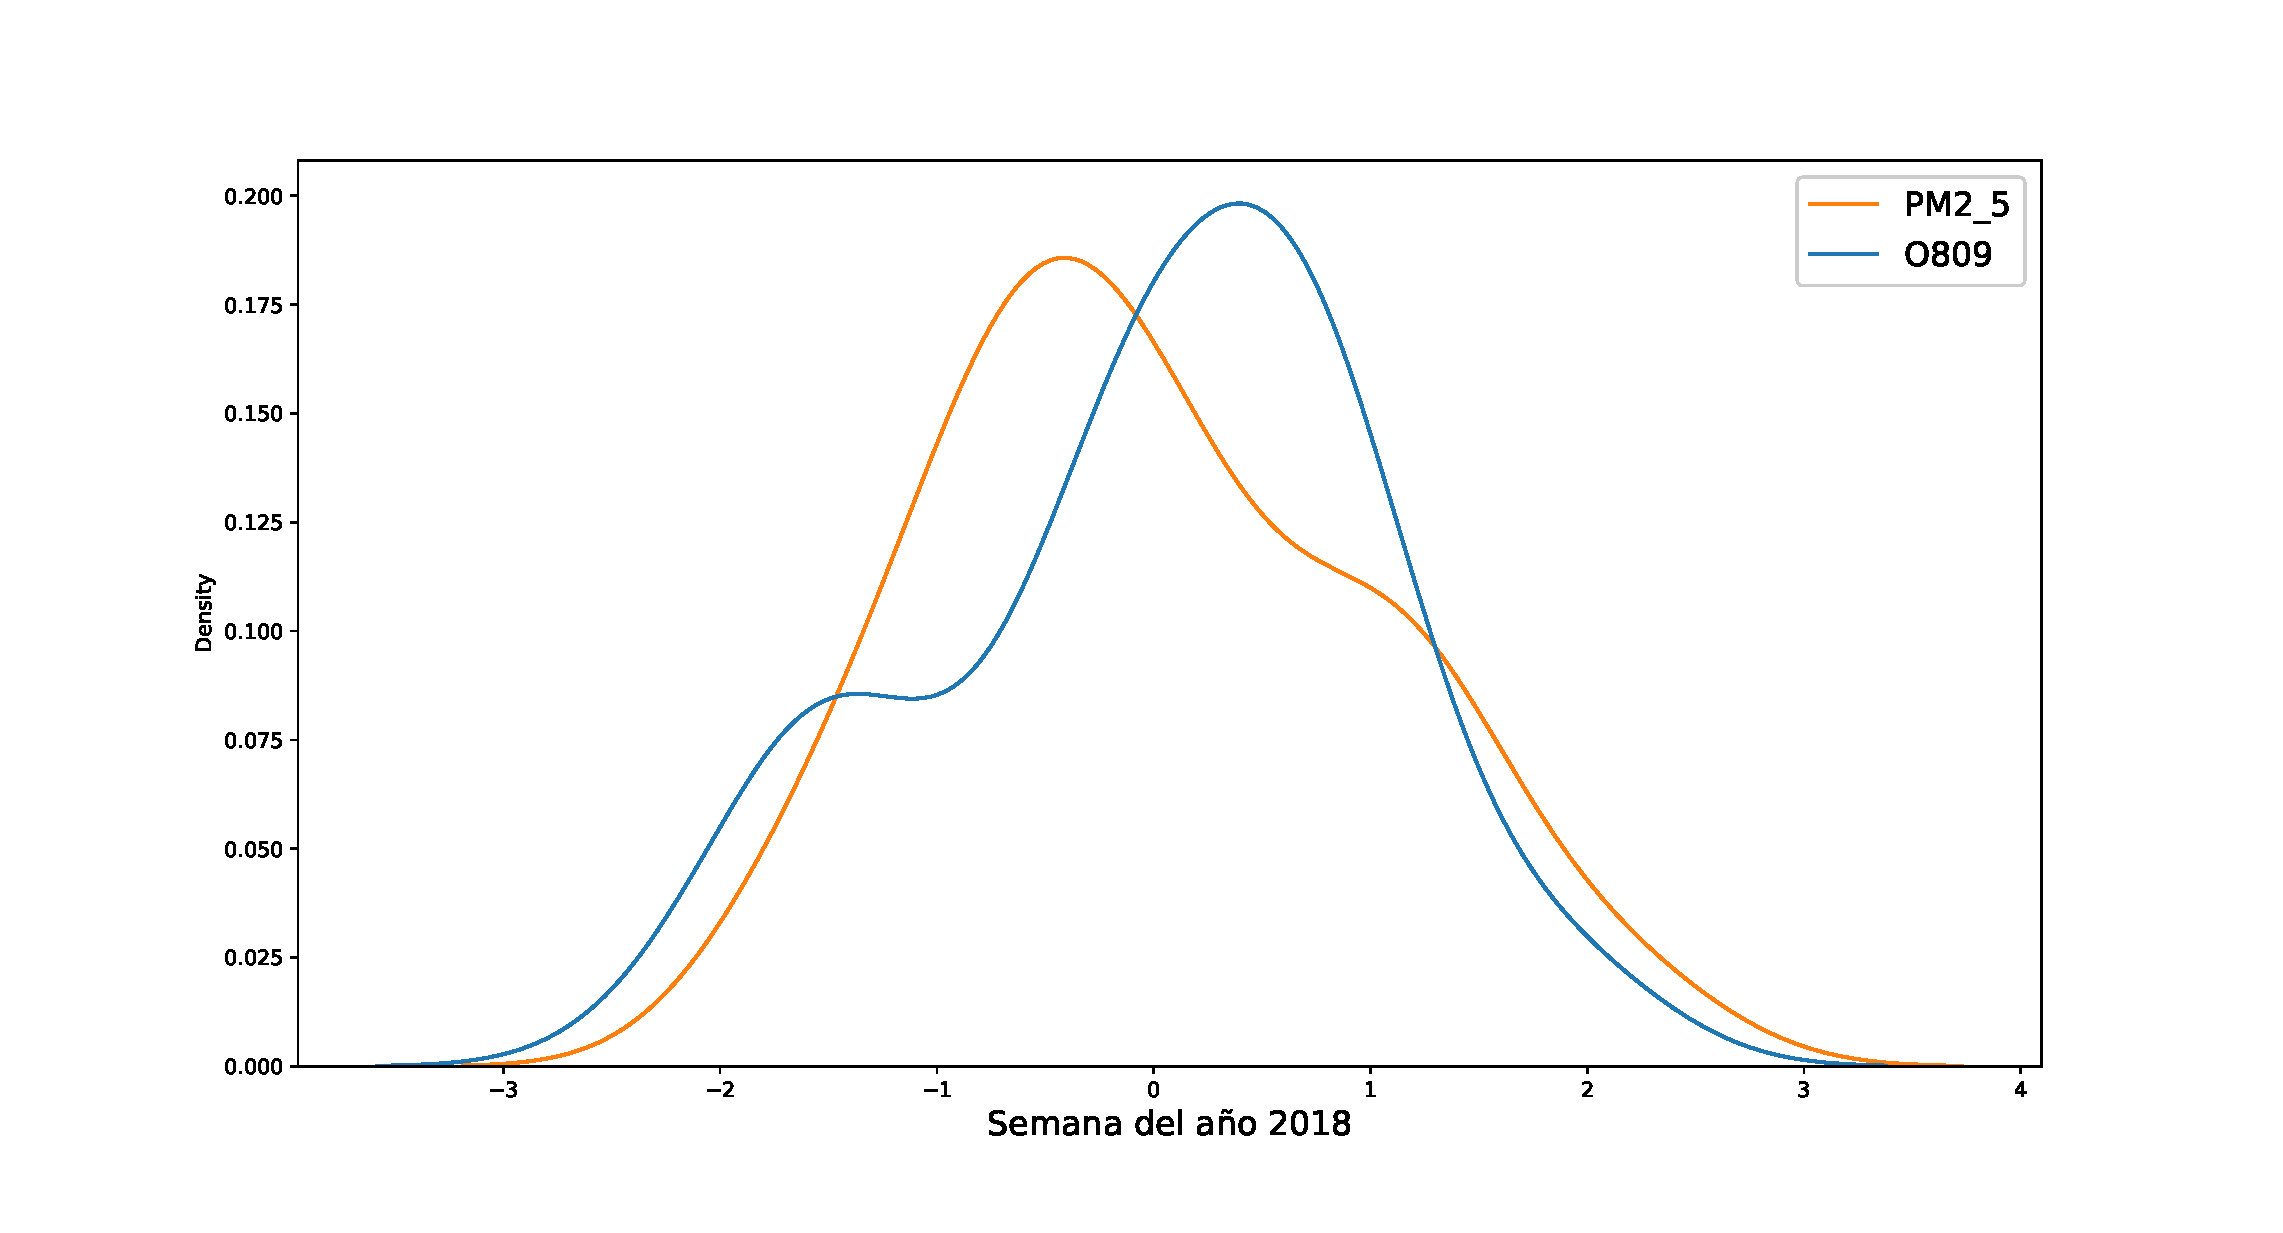
\includegraphics[trim=61 0 0 0,clip,width=1\textwidth]{PM2_5_O809_2018.eps}
   \end{center}
    \caption[Series de tiempo 2018 PM2.5 y O809]{Evolución de los niveles de PM2.5 y el número de egresos diagnosticados con la CIE O809 en el 2018.}
    \label{serie_de_tiempo_2018_PM25}
\end{figure}

\begin{table}[hbt!]
\centering
\caption{Resultados obtenidos PM2.5 2018}
\label{tab:Resultados obtenidos PM2.5 2018}
\vspace{0.5cm}
\begin{threeparttable}
\begin{tabular}{|c|c|c|c|c|}
	\hline
	CIE & $\rho$ & $R^2$ & Valor $p$ & $\epsilon$\\
	\hline
	O809 & -0.354 & 0.057 & 0.133 & 0.259 \\
	\hline
	O829 & 0.225 & 0.046 & 0.177 & 0.256 \\
	\hline
	K802 & 0.273 & 0.089 & 0.058 & 0.159 \\
	\hline
	O342 & -0.443 & 0.149 & 0.013 & 0.245 \\
	\hline
	N40X & -0.074 & 0.001 & 0.842 & 0.241 \\
	\hline
\end{tabular}
\begin{tablenotes}
\footnotesize
\item{$\rho$ = Coeficiente de correlación de Pearson}
\item{$\epsilon$ = RMSE para medir el error}
\end{tablenotes}
\end{threeparttable}
\end{table}

\begin{figure}[h!]
\setcounter{figure}{7} % por culpa de sciposter
\captionsetup{type=figure} % por culpa de sciposter
\begin{center}
   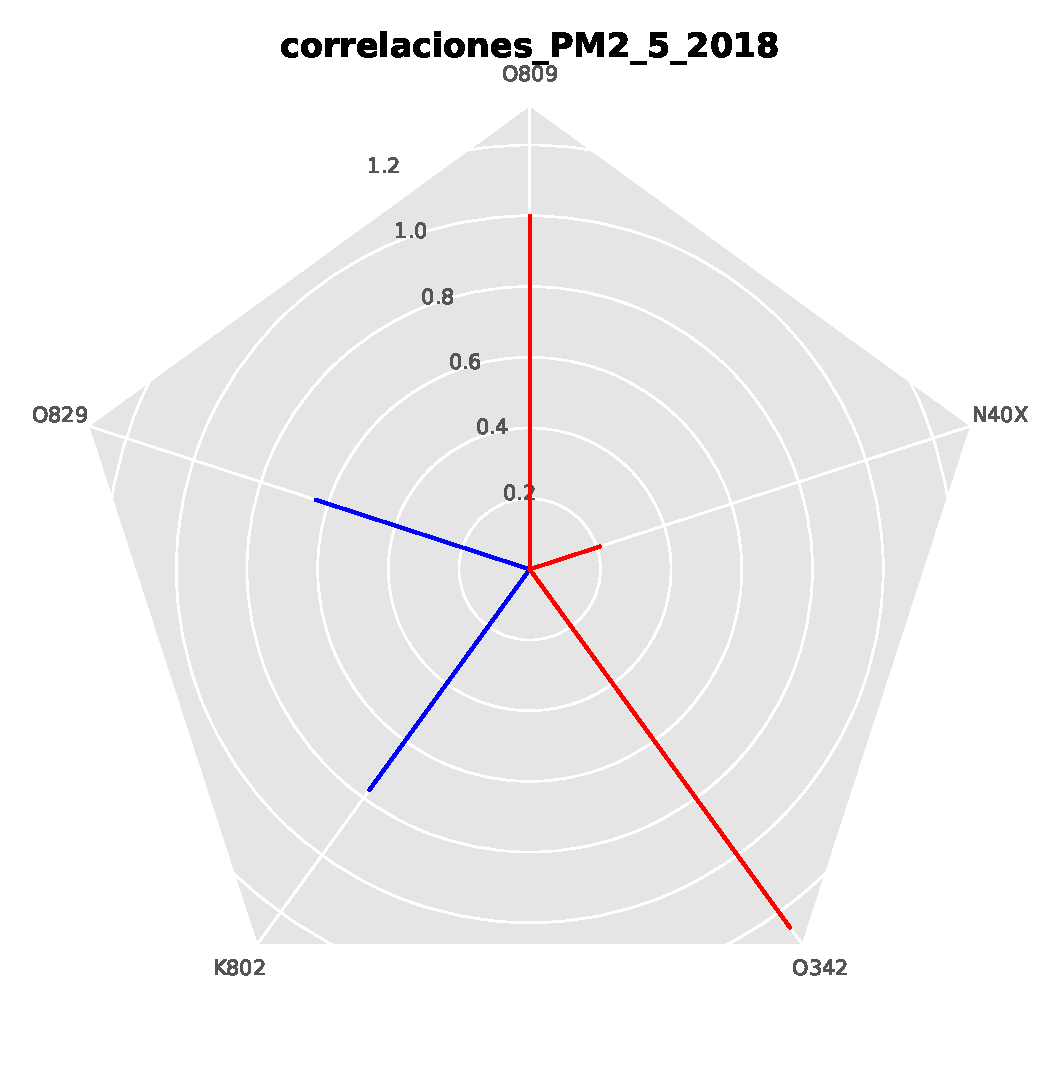
\includegraphics[trim=0 0 0 23,clip,width=1\textwidth]{spiderweb_correlaciones_PM2_5_2018}
   \end{center}
    \caption[Correlaciones 2018 PM2.5]{Correlaciones entre los niveles de PM2.5 y CIE en el 2018 donde el azul indica una correlación positiva y el rojo una correlación negativa.}
    \label{correlaciones_2018_PM25}
\end{figure}

\begin{table}[hbt!]
\caption{Resultados regresión lineal múltiple PM2.5 2018}
\label{tab:RRLM PM2.5 2018}
\begin{center}
\begin{tabular}{lclc}
\toprule
\textbf{Variable Dep.:}    &        $y$         & \textbf{  R$^2$:         } &     0.259   \\
\textbf{Modelo:}            &       OLS        & \textbf{Método:}           &  Mínimos cuadrados   \\
\textbf{Error:}            & 0.174  \\
\bottomrule
\end{tabular}
\begin{tabular}{lcccccc}
               & \textbf{coef} & \textbf{std err} & \textbf{$t$} & \textbf{P$> |$t$|$} & \textbf{[0.025} & \textbf{0.975]}  \\
\midrule
\textbf{const} &       0.7042  &        0.193     &     3.652  &         0.001        &        0.313    &        1.096     \\
\textbf{O809}  &      -0.0863  &        0.172     &    -0.501  &         0.620        &       -0.436    &        0.264     \\
\textbf{O829}  &      -0.1084  &        0.196     &    -0.553  &         0.584        &       -0.507    &        0.290     \\
\textbf{K802}  &       0.3006  &        0.153     &     1.964  &         0.058        &       -0.010    &        0.611     \\
\textbf{O342}  &      -0.3311  &        0.191     &    -1.733  &         0.092        &       -0.719    &        0.057     \\
\textbf{N40X}  &      -0.2053  &        0.154     &    -1.336  &         0.190        &       -0.517    &        0.107     \\
\bottomrule
\end{tabular}
\end{center}
\end{table}


\clearpage
\section{Discusión}
Como se puede observar, en todos los experimentos se obtiene una correlación entre -1 y 1 y diferente a 0, por lo tanto se pueden generar los modelos de regresión lineal.

En el Experimento A el error RMSE en los modelos de regresión lineal varía entre 0.152 y 0.294, lo cual indica que no todos los resultados alcanzan una fiabilidad mayor al 80\%, excepto en la CIE K802 en el año 2018 en la cual se encuentra el porcentaje de error más bajo. 
El valor de $R^2$ más alto en el año 2017 se encuentra en la CIE O759 con un valor $p$ de 0.029, sin embargo, en el modelo de regresión lineal múltiple se encuentra el valor de $R^2$ más alto para el contaminante PM10 en el año 2017. En el año 2018 el valor de $R^2$ más alto se encuentra en la CIE O342 con un valor $p$ de 0.044, sin embargo, en el modelo de regresión lineal múltiple se encuentra el valor de $R^2$ más alto para el contaminante PM10 en el año 2018.

En el Experimento B el error RMSE en los modelos de regresión lineal varía entre 0.159 y 0.278, lo cual indica que no todos los resultados alcanzan una fiabilidad mayor al 80\%, excepto en la CIE K802 en el año 2018 en la cual se encuentra el porcentaje de error más bajo.
El valor de $R^2$ más alto en el año 2017 se encuentra en la CIE O759 con un valor $p$ de 0.032, sin embargo, en el modelo de regresión lineal múltiple se encuentra el valor de $R^2$ más alto para el contaminante PM2.5 en el año 2017. En el año 2018 el valor de $R^2$ más alto se encuentra en la CIE O342 con un valor $p$ de 0.013, sin embargo, en el modelo de regresión lineal múltiple se encuentra el valor de $R^2$ más alto para el contaminante PM2.5 en el año 2018.

\clearpage
Todos los experimentos son ejecutados en \texttt{Jupyter Notebook} en una laptop con las especificaciones del cuadro \ref{tab:Especificaciones técnicas del PC}.

\begin{table}[H]
	{\centering
		\caption{Especificaciones técnicas del equipo de cómputo}
		\begin{tabular}{|c|c|c|}
			\hline
			Sistema Operativo & macOS Big Sur\\
			\hline
			Procesador & Apple M1\\
			\hline
			RAM & 8 GB RAM\\
			\hline
		\end{tabular}

	\label{tab:Especificaciones técnicas del PC}
	}
\end{table}

%\subsection{Experimento C: Niveles de NO$_x$}
%\subsubsection{Año 2015}
%\subsubsection{Año 2016}
%\subsubsection{Año 2017}
%\subsubsection{Año 2018}

%\subsection{Experimento D: Niveles de NO$_2$}
%\subsubsection{Año 2015}
%\subsubsection{Año 2016}
%\subsubsection{Año 2017}
%\subsubsection{Año 2018}
\chapter{Conclusiones}

El presente capítulo describe la tesis a partir de la manera que cumple los objetivos generales y específicos para determinar si la hipótesis se comprueba, trata también del porqué se realizó la tesis.

En el presente proyecto se generaron visualizaciones para el estudio de las relaciones entre determinados contaminantes y determinadas CIE. Además, se generaron modelos de regresión lineal y modelos de regresión lineal múltiple con diferentes contaminantes y diferentes CIE para poder realizar una comparación entre los modelos generados.

En los experimentos se encontró un coeficiente de correlación de Pearson diferente a 0 entre -1 y 1, por lo tanto se pudieron generar los modelos de regresión lineal. Se encontró que al estudiar las CIE de manera agrupada en un modelo de regresión múltiple se obtiene una mejor explicación de la varianza de los niveles de los contaminantes PM10 y PM2.5 frente al modelo de regresión lineal simple. Cinco de los veinticuatro valores de error RMSE reportados son menores a 0.20, lo cual indica que la mayoría de los valores predichos por los modelos se alejaron más de 0.20 unidades de los valores reales, por lo tanto dichos valores de error son mayores a los deseados.

\section{Contribuciones}
Primeramente se encontró que la CIE que reporta mayor número de egresos en Nuevo León, México en los años 2017 y 2018 es la CIE O809. En las series de tiempo se observa que la cantidad de egresos de la mayoría de las CIE estudiadas presentar una línea de evolución similar al contaminante PM10.

Además, se encontró una correlación lineal entre los contaminantes estudiados y las CIE estudiadas, por lo cual el presente proyecto motiva a seguir realizando labores en torno a la investigación de la dependencia lineal que se presenta entre los contaminantes y las CIE.

Finalmente, se observó que para el estudio de las relaciones entre los contaminantes y las CIE se obtuvieron mejores resultados con los modelos de regresión lineal frente a los modelos de regresión lineal simple, lo cual indica que se puede obtener información relevante si se emplean modelos de regresión lineal múltiple para realizar investigaciones que estudien las relaciones entre los niveles de determinados contaminantes y el número de egresos por determinadas CIE.

\clearpage
\section{Trabajo a futuro}
El presente trabajo brinda algunos aspectos a considerar para realizar un trabajo a futuro, los cuales son: la recolección de más datos de los niveles de contaminantes y de egresos para el estudio de años más recientes, realizar un estudio de las relaciones de los niveles de determinados contaminantes y la cantidad de egresos por CIE empleando modelos de regresión lineal múltiple, la creación de un mapa interactivo donde se pueda observar por región los niveles de los contaminantes y la cantidad de egresos, y la generación de una página web que funcione en conjunto con el desarrollo elaborado para que al ingresar el archivo con los datos se generen las visualizaciones y modelos.

Las oportunidades de mejora detectada para el presente proyecto son: comparar los resultados obtenidos de los modelos regresión lineal múltiple con el mismo modelo pero incrementando el número de variables independientes (CIE), elaborar modelos de regresión no lineal para comparar sus resultados con los resultados de los modelos generados, y utilizar un conjunto de datos más consistente ya que eso favorece a que se tengan resultados más fiables y precisos.


% PENDIENTES:
% RESUMEN EN INGLES

\appendix
%%% Haz un documento para cada apéndice
%%\chapter{CIE y sus nombres de enfermedades}

\begin{table}[H]
	{\centering
		\caption{CIE mencionadas en los Experimentos y el nombre de la enfermedad.}
		\begin{tabular}{|c|c|c|}
			\hline 
			CIE & Enfermedad\\
			\hline
			N40-N53 & Enfermedades de los órganos genitales masculino\\
			\hline
			K00-K93 & Enfermedades del aparato digestivo\\
			\hline
			O00-O99 & Embarazo, parto y puerperio\\
			\hline
		\end{tabular}
		
	\label{tab:CIE y sus nombres de enfermedades}
	}
\end{table}


%En princicpio tienes total libertad de incluir tu bibliografía con el entorno {\tt thebibliography} nativo de \LaTeX{} o mediante la herramienta \textsc{Bib}\TeX. En caso de que optes por esto último (recomendado), puedes usar alguno de los archivos {\tt mighelbib.bst} o {\tt mighelnat.bst} incluidos en el paquete {\tt Tesis-FIME}, pues sus diseños están basados en el estilo bibliográfico estándar del español, además de que armoniza con el estilo de tesis provisto por {\tt fime.cls}.

%El estilo bibliográfico {\tt mighelbib} es numérico, es decir cita con un número entre corchetes, por ejemplo una cita \verb+\cite{Dan82}+ genera una etiqueta del tipo [13], mientras que el estilo {\tt mighelnat} es tipo autor-año y requiere que el paquete {\tt natbib} sea cargado (sin opciones) para su correcto funcionamiento, cita con el apellido del autor y el año, por ejemplo una cita \verb+\citet{Dan82}+ genera una etiqueta del tipo Dantzig (1982), mientras que una cita \verb+\citep{Dan82}+ genera una etiqueta del tipo (Dantzig, 1982).

%Como muestra del estilo, unas citas: un libro clásico de programación lineal \cite{Baz04} y un documento histórico \cite{Dan82}. Para saber un poco más del uso de \textsc{Bib}\TeX, se puede leer \cite{Mat11}.

%\section{Comillas}

%El objetivo de esta sección era provocar otra página para que se vea el encabezado. Pero aprovechamos para decir que la clase {\tt fime.cls} carga el paquete {\tt babel} con la opción {\tt spanish}, por lo que cambiará automáticamente los dobles signos $<<$ y $>>$ por << y >>. Estas comillas angulares son las correctas en el idioma español, y son las que se usan en la clase {\tt fime.cls}, por lo que se sugiere sean las usadas en el texto cada que quieras <<entrecomillar>> algo.



\backmatter
\pagestyle{main}

%%% Aquí va la bibliografía, puedes usar el entorno de LaTeX (thebibliography)
%%% o la herramienta BibTeX. En caso de que optes por BibTeX, puedes usar
%%% alguno de los archivos de estilo (mighelbib.bst o mighelnat.bst) incluidos
%%% en el paquete, cuyos diseños armonizan con el diseño de tesis provisto por
%%% fime.cls. Para muestra, basta un botón:
\bibliographystyle{mighelnat}
\bibliography{MiBiblio}

\label{lastpage}
\chapter{CIE y sus nombres de enfermedades}

\begin{table}[H]
	{\centering
		\caption{CIE mencionadas en los Experimentos y el nombre de la enfermedad.}
		\begin{tabular}{|c|c|c|}
			\hline 
			CIE & Enfermedad\\
			\hline
			N40-N53 & Enfermedades de los órganos genitales masculino\\
			\hline
			K00-K93 & Enfermedades del aparato digestivo\\
			\hline
			O00-O99 & Embarazo, parto y puerperio\\
			\hline
		\end{tabular}
		
	\label{tab:CIE y sus nombres de enfermedades}
	}
\end{table}


%En princicpio tienes total libertad de incluir tu bibliografía con el entorno {\tt thebibliography} nativo de \LaTeX{} o mediante la herramienta \textsc{Bib}\TeX. En caso de que optes por esto último (recomendado), puedes usar alguno de los archivos {\tt mighelbib.bst} o {\tt mighelnat.bst} incluidos en el paquete {\tt Tesis-FIME}, pues sus diseños están basados en el estilo bibliográfico estándar del español, además de que armoniza con el estilo de tesis provisto por {\tt fime.cls}.

%El estilo bibliográfico {\tt mighelbib} es numérico, es decir cita con un número entre corchetes, por ejemplo una cita \verb+\cite{Dan82}+ genera una etiqueta del tipo [13], mientras que el estilo {\tt mighelnat} es tipo autor-año y requiere que el paquete {\tt natbib} sea cargado (sin opciones) para su correcto funcionamiento, cita con el apellido del autor y el año, por ejemplo una cita \verb+\citet{Dan82}+ genera una etiqueta del tipo Dantzig (1982), mientras que una cita \verb+\citep{Dan82}+ genera una etiqueta del tipo (Dantzig, 1982).

%Como muestra del estilo, unas citas: un libro clásico de programación lineal \cite{Baz04} y un documento histórico \cite{Dan82}. Para saber un poco más del uso de \textsc{Bib}\TeX, se puede leer \cite{Mat11}.

%\section{Comillas}

%El objetivo de esta sección era provocar otra página para que se vea el encabezado. Pero aprovechamos para decir que la clase {\tt fime.cls} carga el paquete {\tt babel} con la opción {\tt spanish}, por lo que cambiará automáticamente los dobles signos $<<$ y $>>$ por << y >>. Estas comillas angulares son las correctas en el idioma español, y son las que se usan en la clase {\tt fime.cls}, por lo que se sugiere sean las usadas en el texto cada que quieras <<entrecomillar>> algo.


%Autobiografia

\chapter*{Resumen autobiográfico}
\thispagestyle{empty}

\begin{center}
\autor

Candidato para obtener el grado de\\
\grado\\
\orientacion\bigskip

\uanl\\
\fime\bigskip

Tesis:\\
\textsc{\large\titulo}
\end{center}\bigskip

%Aquí va tu historia
Nací el 30 de Junio de 2000 en Monterrey, Nuevo León, soy la mayor de 4 hijos. Mi familia está conformada por mi madre Lilia Prado López, mi padre Adan Alfaro Lerma, y mis hermanos: Angel Alejandro Prado Prado, Estrella Belen Prado Prado, y Genesis Adali Alfaro Prado. \\
Desde pequeña me han gustado las matemáticas, aprender como funcionan los sistemas computacionales, y leer. \\
Durante los primeros semestres de de mi carrera descubrí la inteligencia computacional, un área que me encantó desde que la descubrí, en especial su rama de ciencia de datos, rama en la que espero seguir desarrollandome. \\
Otra cosa que me apasiona es dibujar y pintar, actividades que estaban dentro de mi pero que se avivaron cuando inició la pandemia en el año 2020.

\end{document}